\documentclass[12pt]{book}
\usepackage[utf8]{inputenc}
\usepackage{multicol}
\usepackage{amsthm}
\usepackage{graphicx}
\usepackage{ulem}
\usepackage{wasysym}
\usepackage{array}
\usepackage{enumerate}
\usepackage{hyperref}
\hypersetup{
    colorlinks=true,
    linkcolor=blue,
    filecolor=magenta,
    urlcolor=cyan,
}

\theoremstyle{definition}
\newtheorem{exmp}{Example}[section]
\newcolumntype{C}[1]{>{\centering\let\newline\\\arraybackslash\hspace{0pt}}m{#1}}
\title{Year 9 Mathematics}
\author{Mark Winfield}
\date{\today}

\begin{document}
\maketitle
\tableofcontents

\chapter{Algebra 1}
\section{Notation}
It is importatant that when we see some algebra on the page or board that we all agree what it represents.  In this section we will introduce simply algebraic notation.
\subsection{A letter can have a value}
Imagine that apples come in bags of five that are all the same weight and that on the bag it gives their individual weight.  How would we calculate the total weight of the apples in a bag.  We would multiply the weight by 5. 

We have just described in words how to get the total weight, algebra will allow us to do this in a simplier way.  We can do this by letting 'a' represent the weight of the apple, so now the we get the equation:
$$\mbox{Total Weight} = a \times 5$$
Better still we can let 'T' represent the total weight. We now get:
$$T=a \times 5$$
\subsection{Four rules}

Addition is just what you are used to and is shown with a plus sign (+)

\noindent Subtraction is just what you are used to and is shown with a minus sign (-)
\noindent Multiplication is slightly different.  In algebra we don't use a multiplication sign we just leave it out.  It is understood that if two values are next to each other then we need to multiply them together.

For example:

$5a$ means 5 $\times$ the value of a

$ab$ means the value of a $\times$ the value of b

\noindent Something else to remember with multiplication is that we would usually put the letters in alphabetical order and we would also put numbers first.

So:
$a5$ becomes $5a$

$yx$ becomes $xy$

$x5a$ becomes $5ax$

\noindent So our equation from before becomes $$T = 5a$$

\noindent Division is simply shown as a fraction.  So $\frac{a}{b}$ means $a \div b$
\subsection{Exercise}
Write each of following statements using algebra
\begin{multicols}{2}
\begin{enumerate}
  \item a plus 6
  \item 5 minus b
  \item x multiplied z
  \item t divided by 4
  \item the total of a and b
  \item the difference between 9 and p
  \item g $\times$ 7
  \item \textbf{A equals b multiplied h}
  \item \textbf{I equals V $\div$ R}
  \item \textbf{P equals the total of a, b and c}
  \item t more than q
  \item p less than 8
  \item 4 more than ab
  \item f shared by r
  \item f less than g
  \item g less than f
  \item h less than pq
  \item p times d
  \item \textbf{v equals the total of u and 'at'}
  \item \textbf{A equals bh divided by 2}
\end{enumerate}
\end{multicols}
\section{Substitution}
It this point we understand basic algebraic notation and we also know how to produce basic expressions and equations.  In this section we are going to work out the value of various expressions.  We will be given the value of the letters and we will use these.
\begin{exmp}
What is the value $ab$ if $a=3$ and $b=7$?

$ab$ means $a \times b$

So $ab = 3 \times 7$

So $ab = 21$
\end{exmp}
\begin{exmp}
Given that $a= 4$, $b = 6$ and $c= 5$, what is $P$ if $P=a+b+c$?

$P=4+6+5$

So $P=15$
\end{exmp}
\subsection{Exercise}
Find the value of the following expressions given that $a=3,b=6,c=5,d=10,h=4$
\begin{multicols}{2}
\begin{enumerate}
  \item $a+b$
  \item $5b$
  \item $a + b + c + d$
  \item $bh$
  \item $\displaystyle \frac{d}{c}$
  \item $d-h$
  \item $\displaystyle \frac{15}{a}$
  \item $12 - c$
  \item $\displaystyle \frac{d}{2}$
  \item $7+h$
\end{enumerate}
\end{multicols}
Find the value of $x$ using the following equations.
\begin{multicols}{2}
\begin{enumerate}
  \setcounter{enumi}{10}
  \item $x=7a$
  \item $x=8+c$
  \item $x=b+d$
  \item $x=abc$
  \item $\displaystyle x=\frac{18}{a}$
  \item $d+h$
\end{enumerate}
\end{multicols}
\section{Codes}
In this section we are going read a code that has been given as a series of expressions.  We will calculate the value of the expressions and then use the talbe to find out to what letter we are refering.  For example if the value of an expression is '13' we can see from the table that this must represent a 'C'.


\begin{tabular}{|c|c|c|c|c|c|c|c|c|c|c|c|c|}
  \hline
  A & B & C & D & E & F & G & H & I & J & K & L & M \\
  \hline
  7 & 5 & 13 & 35 & 1 & 42 & 63 & 3 & 9 & 2 & 12 & 30 & 27\\
  \hline
  \hline
  N & O & P & Q & R & S & T & U & V & W & X & Y & Z\\
  \hline
  0 & 4 & 33 & 11 & 6 & 8 & 10 & 21 & 25 & 13 & 22 & 18 & 28\\
  \hline
\end{tabular}

\begin{exmp}
Given that $a= 3$, $b = 15$, $c= 1$ and $d = 21$ change each line of the table into a word to decode the message.

\vspace{3 mm}

\renewcommand{\arraystretch}{3}
\begin{tabular}{|c|c|c|c|}
\hline
$a + 2$ & $b - 6$ & $3d$ &  \\
\hline
$\displaystyle\frac{b}{a}$ & $\displaystyle\frac{d}{a}$ & $20 - b$ & $a + b$ \\
\hline
\end{tabular}

\vspace{3 mm}

Let's substitute in the values

\vspace{3 mm}

\begin{tabular}{|c|c|c|c|}
\hline
$3 + 2 = 5$ & $15 - 6 = 9$ & $3 \times 21 = 63$ &  \\
\hline
$\displaystyle \frac{15}{3} = 5$ & $\displaystyle \frac{21}{3} = 7$ & $20 - 15 = 5$ &$3 + 15 = 18$ \\
\hline
\end{tabular}

\vspace{3 mm}

Change for the letters

\vspace{3 mm}

\renewcommand{\arraystretch}{1}
\begin{tabular}{|c|c|c|c|}
\hline
B & I & G &  \\
\hline
B & A & B & Y \\
\hline
\end{tabular}

\vspace{3 mm}

So the message is 'Big baby'.
\end{exmp}
\pagebreak
\subsection{Exercise}
\begin{tabular}{|c|c|c|c|c|c|c|c|c|c|c|c|c|}
  \hline
  A & B & C & D & E & F & G & H & I & J & K & L & M \\
  \hline
  7 & 5 & 13 & 35 & 1 & 42 & 63 & 3 & 9 & 2 & 12 & 30 & 27\\
  \hline
  \hline
  N & O & P & Q & R & S & T & U & V & W & X & Y & Z\\
  \hline
  0 & 4 & 33 & 11 & 6 & 8 & 10 & 21 & 25 & 13 & 22 & 18 & 28\\
  \hline
\end{tabular}

\vspace{3 mm}
\noindent Given that 
\begin{multicols}{3}
	\begin{itemize}
		\item $p = 50$
		\item $q = 27$
		\item $r = 9$
		\item $s = 15$
		\item $t = 3$
		\item $u = 2$
		\item $v = 10$
		\item $w = 24$
		\item $x = 7$
	\end{itemize}
\end{multicols}
\noindent change each line of the table into a word to find the name of this cartoon character.

\vspace{3 mm}

\renewcommand{\arraystretch}{3}
\begin{tabular}{|c|c|c|c|c|}
\hline
$\displaystyle \frac{s}{t}$ & $v - r$ & $x + t$ & $q - x - v$ & $2r$ \\
\hline
$\displaystyle \frac{p}{v}$ & $2u$ & $\displaystyle \frac{w}{6}$ & $p - q + v$& \\
\hline
\end{tabular}

\vspace{3 mm}


\chapter{Number 1}
\section{Integers}
An integer is just a whole number, it does not have digits after the decimal point and it is not a fraction.  Early mathematics used some of these number to solve the kinds of problems that were important to the people of the day, like counting sheep or the number of days etc.
\section{Four Rules}
\subsection{Additition}
When we want to add two and three digit numbers together we follow an algorithm, a set of instructions.  If we follow these instructions correctly we will end up with the desired result.  Let's look at an algorithm for adding two numbers together.  We will first look at it displayed as a flow chart and then given as a series of steps:

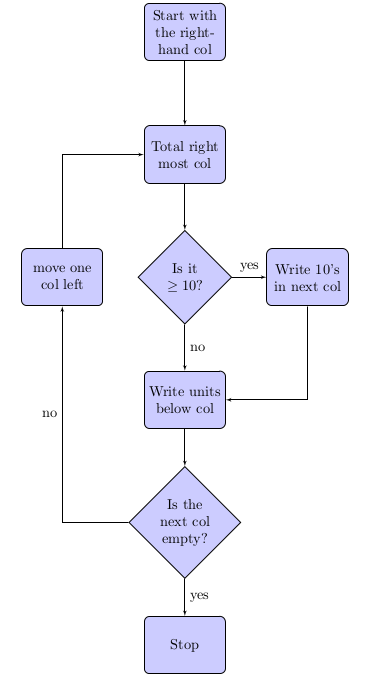
\includegraphics[width=15cm,height=15cm,keepaspectratio]{./Images/Number/Flow1}

\begin{enumerate}
	\item Write down the numbers lining up the digits by place value (i.e. units under units)
	\item Find the total of the right most column that has not already been totaled
	\item If the total is $> 10$ then write the tens part in the next column to the left
	\item Write down the units value
	\item If the next column is empty. STOP
	\item Go to step 2.
\end{enumerate}

\begin{exmp}
What is $256+28$?
Step 1. Write the numbers down, lining up the columns.

\renewcommand{\arraystretch}{1}
\begin{tabular}{c c c}
	2 & 5 & 6 \\
	  & 2 & 8 \\
	\hline \hline
	  &   &   \\
\end{tabular}

The right-hand column has a total of 14, that is 1 ten and 4 units.  We will now put the 1 in the next column and the 4 below the column we have just totaled.

\renewcommand{\arraystretch}{1}
\begin{tabular}{c c c}
	2 & 5 & 6 \\
	  & 2 & 8 \\
	\hline \hline
	  & $^1$  & 4 \\
\end{tabular}
\end{exmp}

The next column is not empty so let's find its total.
The total is 8 (don't forget the 1), so we have nothing to put in the next column, just 8 in this one.

\renewcommand{\arraystretch}{1}
\begin{tabular}{c c c}
	2 & 5 & 6 \\
	  & 2 & 8 \\
	\hline \hline
	  & $8^1$  & 4  \\
\end{tabular}

The next column is not empty so let's find its total.
The total is 2, so we have nothing to put in the next column, just 2 in this one.

\renewcommand{\arraystretch}{1}
\begin{tabular}{c c c}
	2 & 5 & 6 \\
	  & 2 & 8 \\
	\hline \hline
	2  & $8^1$  & 4  \\
\end{tabular}

The next column is empty so we have finished.  The answer is 284.
\subsection{Exercise}
Find the answers to the questions below, do not use a calculator:
\begin{multicols}{2}
\begin{enumerate}
  \item $45 + 28$
  \item $295 + 21$
  \item $462 + 352$
  \item $652 + 347$
  \item $147 + 345 + 252$
  \item $359 + 875$
  \item What is the total cost of a car at \$3457 and a boat at \$5385?
  \item What is the cost of a dog at \$299 and a cat at \$145?
  \item How much would it cost for a \$45 hat a \$72 shirt and a \$164 coat?
  \item The flight for a holiday is \$572 and the accomodation is \$365.  What is the total price?
  \item One boy has 864\cent \hspace{1 mm} and another has 395\cent, how much have they got in total?
  \item Fred has 28 apples, Timmy has 110 tomatoes and Steve has 2247 pears. How many fruits do they have altogether? (A.T.)
  \item A flight to Hong Kong costs \$396 per child, \$626 per adult and \$530 per student. How much would it cost for 2 adults, a child and a student to fly to Hong Kong? (I.F.)
  \item Frank wants to buy a \$39 pair of trousers a \$72 jacket and a \$16 burrito for lunch. How much is that in total? (C.C.S.)
  \item If you ate a slice of pizza that weighed 758 grams and a cookie that weighed 425 grams how much would you have eaten. (J.P.)
  \item How much would it cost if 100 doughnuts are \$245 and 80 waffles are \$193? (P.O.B.)
  \item What is the total cost of a mohawk haircut at \$53 and red hair dye at \$168? (L.G.)
  \item Jeboris spent \$4378 on a car and then \$950 on a new phone, how much did he spend in total? (J.L.)
  \item If Bill was in an aeroplane that travelled up 1874 metres and then another 297 metres, how far up would he be? (I.B.)
  \item Billy won a lotto of \$186944 in march. Later in April billy won a lotto of \$794999.  How much money would billy have if he combined all his lotto money together? (A.S)
\end{enumerate}
\end{multicols}
\subsection{Subtraction}
To subtract one number from another we can again follow an algorithm, but first we must learn how to \textbf{decompose/recompose} a number.
\noindent Let's consider the number $3053$ and look at all the different ways we can write it that will be useful for subtraction.

\renewcommand{\arraystretch}{1}
\begin{tabular}{| c | c | c | c |}
	\hline
	3 & 0 & 5 & 3 \\
	\hline
	3 & 0 & 4 & 13 \\
	\hline
	2 & 9 & 15 & 3 \\
	\hline
	2 & 10 & 5 & 3\\
	\hline
\end{tabular}

The first change makes the units column 10 bigger and the tens column 1 smaller.

The second change makes the tens column 10 bigger, but because the hundreds column is contains a zero we must make the number that makes up the thousands and hundreds columns 1 smaller.

The third change makes the hundreds column 10 bigger and the thousands column 1 smaller.

In each case we made the column to the right 10 bigger and the column, or if there were zeros present, columns to the left 1 smaller.

This technique will be important because we can only take a smaller number from a bigger one.

The algorithm
\begin{enumerate}
  \item Write down the two numbers lining up the digits
  \item Start at the right-hand column
  \item If the upper digit is larger than the lower digit then do the subtraction and write the number underneath
  \item If not, decompose/recompose the upper number so that the upper digit is 10 bigger
  \item move one column to the left
  \item repeat until the last column has been calculated
\end{enumerate}

\begin{exmp}
What is $342 - 227$?

\renewcommand{\arraystretch}{1}
\begin{tabular}{c c c}
	3 & 4 & 2 \\
	2 & 2 & 7 \\
	\hline \hline
	 & & \\
\end{tabular}

The 2 is smaller than the 7 so we will make it 10 bigger and the 4 we will make 1 smaller.

\begin{tabular}{c c c}
	3 & 3 & $^1 2$ \\
	2 & 2 & 7 \\
	\hline \hline
	 & & \\
\end{tabular}
We can now do the subtraction in this column.

\begin{tabular}{c c c}
	3 & 3 & $^1 2$ \\
	2 & 2 & 7 \\
	\hline \hline
	 & & 5\\
\end{tabular}

You should be able to see that we can now do the next two columns

\begin{tabular}{c c c}
	3 & 3 & $^1 2$ \\
	2 & 2 & 7 \\
	\hline \hline
	1 & 1 & 5\\
\end{tabular}

The the answer is 115.
\end{exmp}

\subsection{Exercise}
Find the answers to the questions below, do not use a calculator:
\begin{multicols}{2}
\begin{enumerate}
  \item $45 - 28$
  \item $295 - 21$
  \item $462 - 356$
  \item $652 - 347$
  \item $305 - 258$
  \item $914 - 655$
  \item A car on an online auction site costs \$658, we have \$894.  If we buy the car how much money will we have left?
  \item If one tree if 267cm tall and another is 385cm tall, what is the difference between their heights?
\end{enumerate}
\end{multicols}
\noindent The next few questions will require you use your understanding of previous sections of the book
\begin{enumerate}
	\setcounter{enumi}{8}
	\item Kite has 145\cent  \ and her brother has 372\cent.  If they put their money together and buy sweets costing 415\cent, how much change will they have?
	\item Esme has two pieces of wood, one 376cm long the other is 448cm long.  She wants to join them together to make a piece which is 525cm long  How much wood will she have left?
\end{enumerate}

\subsection{Multiplication}
There are many different algorithms that we can use to multiply two numbers together, in this book we will use the lattice method.  You might have another method that you prefer.

Let's show how this works by using an example.
\begin{exmp}
	What is $234 \times 56$?

	Since we are multiplying a three digit number by a two digit number we draw a 3 by 2 grid with the numbers lined up on the outside.

	\begin{center}
	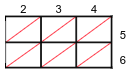
\includegraphics[height=2.1cm,keepaspectratio]{./Images/Number/mult1}
	\end{center}

	We start by treating our grid as a multiplication table.  Let's consider the last column and the bottom row ($4 \times 6$ which is $24$.  We put the ten's part (2) on the left side of the box and the unit's part (4) on the right side.

	\begin{center}
	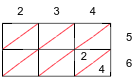
\includegraphics[height=2.1cm,keepaspectratio]{./Images/Number/mult2}
	\end{center}

	Let's fill out the rest of grid.

	\begin{center}
	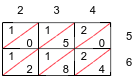
\includegraphics[height=2.1cm,keepaspectratio]{./Images/Number/mult3}
	\end{center}

	We now add up the values in each diagonal carry tens if required to get our answer.

	\begin{center}
	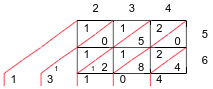
\includegraphics[height=2.5cm,keepaspectratio]{./Images/Number/mult4}
	\end{center}
\end{exmp}

\subsection{Exercise}
Find the answers to the questions below, do not use a calculator:
\begin{multicols}{2}
\begin{enumerate}
  \item $234 \times 55$
  \item $103 \times 27$
  \item $502 \times 16$
  \item $8625 \times 61$
  \item $492 \times 222$
  \item $195 \times 195$
\end{enumerate}
\end{multicols}
\begin{enumerate}
	\setcounter{enumi}{6}
	\item What is the weight of 27 bags each weighing 375g?
	\item A year group has 117 students who are 13 years old and 156 who are 14 years old.  What is the combined number of years that they have lived?
\end{enumerate}
\noindent The next few questions will require you use your understanding of previous sections of the book
\begin{enumerate}
	\setcounter{enumi}{8}
	\item A lift can carry a total weight of 950kg.  If 13 women enter the lift with weights all around 69kg, how much stuff can they carry with them before the lift becomes dangerous?
	\item On a road trip Esm\'e drives 45km a day for 27 days and Alex then drives 107km a day for 11 days.  How far do they travel altogether?
\end{enumerate}

\subsection{Division}
There are many ways to divide one number into another, we will use the method of short division.  One big difference with division is that we work from the left-hand column rather than the right-hand side.  The skills that we will require are division of single digit numbers and finding the remainder.

Let's see how this works using an example.

\begin{exmp}
What is $375 \div 5$?

First we need to set up our calculation area.  The answer will go above the line.
\begin{center}
\begin{tabular}{c  C{0.4cm} C{0.4cm} C{0.4cm}}
\cline{2-4}
\multicolumn{1}{c|}
5 & 3 & 7 & 5 \\
\end{tabular}
\end{center}

Now we check to see how many 5's go into 3, the value in the first column.  The answer is 0 so that goes on the answer line and the remainder of 3 goes over to the next column. This changes the 7 to 37.
\begin{center}
\begin{tabular}{c  C{0.4cm} C{0.4cm} C{0.4cm}}
 & 0 &  & \\
\cline{2-4}
\multicolumn{1}{c|}
5 & 3 & $^3$7 & 5 \\
\end{tabular}
\end{center}
Now we check how many 5's go into 37, the value now in the second column.  The answer is 7 so that goes on the answer line and the remainder of 2 goes over to the next column.  This changes the 5 to 25.

\begin{center}
\begin{tabular}{c  C{0.4cm} C{0.4cm} C{0.4cm}}
 & 0 & 7 & \\
\cline{2-4}
\multicolumn{1}{c|}
5 & 3 & $^3$7 & $^2$5 \\
\end{tabular}
\end{center}

Finally we check to see how many 5's go into 25.  The answer is 5 and that goes on the answer line.  There is no remainder.
\begin{center}
\begin{tabular}{c  C{0.4cm} C{0.4cm} C{0.4cm}}
 & 0 & 7 & 5\\
\cline{2-4}
\multicolumn{1}{c|}
5 & 3 & $^3$8 & $^2$5 \\
\end{tabular}
\end{center}

So $375 \div 5 = 75$
\end{exmp}

\subsection{Exercise}
Find the answers to the questions below, do not use a calculator:
\begin{multicols}{2}
\begin{enumerate}
	\item $216 \div 6$
	\item $681 \div 3$
	\item $5475 \div 5$
	\item $18599 \div 7$
	\item $292 \div 4$
	\item $8532 \div 9$
\end{enumerate}
\end{multicols}
If when we have got past the last column we still have a remainder, that is what is left over after the division.
Find the remainder, if there is one for the questions below:
\begin{multicols}{2}
\begin{enumerate}
	\setcounter{enumi}{6}
	\item $1544 \div 7$
	\item $557 \div 8$
	\item $7632 \div 3$
	\item $5316 \div 9$
\end{enumerate}
\end{multicols}

\begin{enumerate}
	\setcounter{enumi}{10}
	\item $531645$ can be divided by $9$ with no remainder.  Change the order of the digits in $531645$ and see what the remainder is now.  What do you notice.
\end{enumerate}
\noindent The next few questions will require you use your understanding of previous sections of the book
\begin{enumerate}
	\setcounter{enumi}{11}
	\item A group of 25 friends decide to share their sweets, they have about 15 each.  When another five friends comes along they decide still share they equally between everyone.  About how many sweets does each friend recieve?
\end{enumerate}

\section{Directed numbers}
Numbers can be positive or negative, because we are using the sign we call them directed numbers.  Let's consider what happens when we add directed numbers together.  Imagine that you have two bank accounts, one of them has \$15 in it and the other has -\$10 dollars in it.  If we were to add these accounts together we would have one account with \$5 in it.  So when we added the negative 10, we just subtracted 10.

\bigskip

Rule 1: When we add a negative we subtract, so $a + -b$ becomes $a - b$

\bigskip

By using the same method above we can easily convince ourselves of rule two.

\bigskip

Rule 2: When we add a positive we add, so $a + +b$ becomes $a + b$

\bigskip

Rules 3 and 4 are wo do with when we subtract directed numbers.

Like before we have two accounts, one with \$15 and one with -\$10.  We know that we have \$5 over all.  Know let's take away the account with \$15 in it, we now have a total of -\$10.  So taking away a positive values was just like subtracting.

\bigskip

Rule 3: When we subtract a positive we subtract, so $a - +b$ becomes $a - b$

\bigskip

Now let's take away the account with -\$10 in it, our balance has go up to \$15.  So take away a negative is like adding.

\bigskip

Rule 4: When we subtract a negative we add, so $a - -b$ becomes $a + b$

\bigskip

An easy way to remember these rules is that if the two signs are the same we add, if they are different we subtract.

\begin{exmp}
Calculate the following:
\begin{enumerate}
	\item $8 + -5$
	\item $7 + +6$
	\item $3 - -7$
	\item $15 - +4$
\end{enumerate}

Answers:
\begin{enumerate}
	\item $8 + -5$ becomes $8 - 5 = 3$
	\item $7 + +6$ becomes $7 + 6 = 13$
	\item $3 - -7$ becomes $3 + 7 = 10$
	\item $15 - +4$ becomes $15 - 4 = 11$
\end{enumerate}
\end{exmp}

\subsection{Exercise}
Find the answers to the following:
\begin{multicols}{2}
\begin{enumerate}
	\item $5 + -1$
	\item $36 + -6$
	\item $17 + +3$
	\item $-1 + +10$
	\item $7 - -10$
	\item $25 - +8$
	\item $23 - -23$
	\item $5 - +12$
\end{enumerate}
\end{multicols}

We will now look at how to multiply and divide directed numbers.
The proofs of these rules will be given in a later algebra section.
The size of the number is calculated by multiply/dividing the number parts, we just use rules 5 and 6 to work out the sign of the answer.

\bigskip

Rule 5: When we multiply/divide to numbers together with the same sign the answer is positive.

\bigskip

Rule 6: When we multiply/divide to numbers together with different signs the answer is negative.

\bigskip

\begin{exmp}
\begin{enumerate}
	\item $-8 \times -5$
	\item $6 \times +4$
	\item $-4 \times +3$
	\item $9 \times -2$
\end{enumerate}

Answers:
\begin{enumerate}
	\item $-8 \times -5$, the answer is positive and $8 \times 5 = 40$ so we get 40
	\item $6 \times +4$, the answer is positive and $6 \times 4 = 24$ so we get 24
	\item $-4 \times +3$, the answer is negative and $4 \times 3 = 12$ so we get -12
	\item $9 \times -2$, the answer is negative and $9 \times 2 = 18$ so we get -18
\end{enumerate}
\end{exmp}

\subsection{Exercise}
Calculate the following:
\begin{multicols}{2}
\begin{enumerate}
	\item $-4 \times -6$
	\item $5 \times -5$
	\item $8 \times +3$
	\item $-13 \times -4$
	\item $4 \times -7$
	\item $-3 \times -9$
\end{enumerate}
\end{multicols}
\section{Factors}
The factors of a number are the whole numbers that divide into the number leaving no remainder.  So, for example, the factors of 10 are 1, 2, 5 and 10.  Again we will use an algorithm to find all the factors of a number.  This is important because it is easy to think that we have them all and to have missed some out.
The algorithm
Let's find the factors of some number N
We what to find all the ways of writing $a \times b = N$ where a and b are integers and $a < b$
\begin{enumerate}
	\item Start with $a=1$
	\item Let $b = N \div a$
	\item If b is a whole number write down $a \times b$
	\item Add 1 to a
	\item If a has already been written down, STOP you have all the factors.
	\item Goto step 2
\end{enumerate}

\begin{exmp}
Find the factors of 28

Try 1: so $1 \times 28$

Try 2: so $2 \times 14$

Try 3: Dividing by 3 leaves a remainder

Try 4: so $4 \times 7$

Try 5: Dividing by 5 leaves a remainder

Try 6: Dividing by 6 leaves a remainder

Try 7: We already have 7 so let's stop.

The factors in order of size are 1, 2, 4, 7, 14, 28

We could have written this as:

\begin{tabular}{c}
28 \\
\hline
$1 \times 28$ \\
$2 \times 14$ \\
$4 \times 7$ \\
\end{tabular}
\end{exmp}

\subsection{Exercise}
Find the factors all the numbers from 1 to 20.  Make a note of how many factors each one has.

\section{Multiples}
The multiples of a number are the values in its times table.  So since the first five values in the 3 times table are 3, 6, 9, 12, 15 then the first five multiples of 3 are 3, 6, 9, 12 and 15.
\begin{exmp}
Find the first four multiples of 7:

$1 \times 7 = 7$

$2 \times 7 = 14$

$3 \times 7 = 21$

$4 \times 7 = 28$

So the first four multiples of 7 are 7, 14, 21 and 28.
\end{exmp}
\begin{exmp}
What is the 10th multiple of 8.

$10 \times 8 = 80$

The 10th multiple of 8 is 80.
\end{exmp}
\subsubsection{Generating a sequence of multiples from a formula}
Let's consider the function $y=3x$
Now let $x$ = whole number values starting at 1.

\begin{tabular}{c|c}
x & y \\
\hline
1 & 3 \\
2 & 6 \\
3 & 9 \\
4 & 12
\end{tabular}

We can see that the y column has given us the multiples of 3.  So we could say that a formula for generating the multplies of 3 is $y=3x$.

\subsection{Exercise}
For the following numbers find the first five multiples, the formula for generating the multiples and the value of the $20^{th}$ multiple.

\begin{enumerate}
	\item 5
	\item 7
	\item 2
	\item 3
	\item 10
	\item 12
\end{enumerate}
\subsection{HCF and LCM}
The Highest Common Factor (HCF) of two numbers is the largest number that is a factor of both numbers.  The Lowest Common Multiple (LCM) of two numbers if the smallest number that is a multiple of both numbers.
\begin{exmp}
Find the HCF of 12 and 16

The factors of 12 are 1, 2, 3, 4, 6, 12

The factors of 16 are 1, 2, 4, 8, 16

The largest number that appears in each list is 4,

So the HCF of 12 and 16 is 4.
\end{exmp}
\begin{exmp}
Find the LCM of 12 and 15

We will work with the largest number.

Does 12 go into 15? No.

Does 12 go into 30? No.

Does 12 go into 45? No.

Does 12 go into 60? Yes.  So the LCM of 12 and 15 is 60.
\end{exmp}
\subsection{Exercise}
For each pair of numbers below find their HCF and LCM
\begin{enumerate}
	\item 6 and 8
	\item 10 and 15
	\item 6 and 9
	\item 12 and 10
	\item 5 and 7
	\item 10 and 20
	\item 4, 6 and 10
\end{enumerate}
Solve the following word problems using L.C.M. or H.C.F.
\begin{enumerate}
	\setcounter{enumi}{7}
	\item Isobel and Anuha are shelving books at a public library. Isobel shelves 5 books at a time, whereas Anuha shelves 6 at a time. If they end up shelving the same number of books, what is the smallest number of books each could have shelved?
	\item Sam and Rose are making emergency-preparedness kits to share with friends. They have 20 bottles of water and
12 cans of food, which they would like to distribute equally among the kits, with nothing left over. What is the greatest number of kits Sam and Rose can make?
	\item Kate has 16 blue marbles and 8 white ones. If she wants to place them in identical groups without any marbles left over, what is the greatest number of groups Kate can make?
	\item Lucas is making trail mix out of 18 bags of nuts and 9 bags of dried fruit. He wants each new portion of trail mix to be identical, containing the same combination of bags of nuts and bags of dried fruit, with no bags left over. What is the greatest number of portions of trail mix Lucas can make?
	\item Isabelle has swimming lessons every fifth day and diving lessons every third day. If she had a swimming lesson and a diving lesson on May 5, when will be the next date on which she has both swimming and diving lessons?
	\item To encourage public transportation, Nathaniel and Guiliana want to give some friends envelopes with bus tickets and train tickets in them. If they have 18 bus tickets and 12 train tickets to split equally among the envelopes, and want no tickets left over, what is the greatest number of envelopes Nathaniel and Guiliana can make?
\end{enumerate}
\section{Decimals}
\subsection{Addition and Subtraction}
To Add and subtract decimals we can use the same methods that we use for integers, all we need to do is make sure that we line up the decimal points in the question and the answer.
\subsection{Exercise}

Find the answers to the questions below (show your working), do not use a calculator:
\begin{multicols}{2}
\begin{enumerate}
	\item $23.6 + 34.2$
	\item $473.3 + 34.8$
	\item $345.5 - 152.3$
	\item $45.46 - 28.54$
	\item $68.46 + 23.35$
	\item $2.625 - 1.526$
	\item $35.6 + 3.56$
	\item $35.6 - 3.56$
	\item $123 + 35.2$
	\item $362 - 94.4$
\end{enumerate}
\end{multicols}
\begin{enumerate}
\setcounter{enumi}{10}
	\item A ball costs \$15.45 and we buy it with a \$20 note.  What is the change?
	\item An alloy is made of 35.9g of iron and 0.25g of tungsten.  What is the total weight?
\end{enumerate}
\subsection{Multiplication}
The important thing to remember when we are multipling decimals together is that the total number of digits after the decimal points in the question is equal to the number of digits after the decimal point in the answer.

So to calculate $23.4 \times 1.02$ we first calculate $234 \times 102$ using any pencil and paper method (23868).  Now since we have a total of three digits after the decimal points in the question we will have three in the answer, so the answer is $23.868$

\subsection{Exercise}
\begin{multicols}{2}
\begin{enumerate}
	\item $25.6 \times 7.4$
	\item $0.5 \times 0.7$
	\item $0.23 \times 0.96$
	\item $7.23 \times 6$
	\item $8.45 \times 75.3$
	\item $4.3 \times 5.34$
	\item $3.45 \times 8.2$
	\item $7.25 \times 0.8$
\end{enumerate}
\end{multicols}
\subsection{Division}
The only extra skill that we need when dividing decimals is that of multiplying by powers of 10 (10, 100, 1000, etc).  If we multiply by a power of 10 the digits stay the same but they move a number places compared to the decimal point equal to the number of zeros after the 1.

So, for example, $4.7 \times 10 = 47$ and $0.13 \times 100 = 13$

In each case here we have turned our decimal into an integer by matching the number of digits after the decimal point to the number of zeros after the 1.

\subsubsection{Method}
\begin{enumerate}
	\item Make sure the number we are dividing by is an integer.  If it is not multiply both numbers by a power of 10 big enough to make it so.
	\item Do the division in the same way as integer division.
	\item If the number we are dividing is a decimal we just have to line up the decimal point in the answer with the one in the question.
\end{enumerate}

So $235.6 \div 0.7 = 2356 \div 7$

\subsection{Exercise}
Calculate:
\begin{enumerate}
	\item $235.6 \div 8$
	\item $235.6 \div 0.8$
	\item $23.56 \div 0.8$
	\item $23.56 \div 0.08$
	\item $235.6 \div 0.08$
	\item $1 \div 7$ find the first 4 digits after the decimal point
	\item $0.053 \div 0.4$
	\item $15 \div 8$ continue until there are no remainders.
\end{enumerate}
\section{Fractions}
A fraction is a division.  It is not a coincidence that a division sign is a dot over a dot and a fraction is a number over a number.  A fraction is always an integer divided by an integer.

\subsection{Fractions to Decimals}
To change a fraction to a decimal we simply divide the numerator (top number) by the denominator (bottom number)
\begin{exmp}
	Change $\frac{4}{5}$ to a decimal.

	$\frac{4}{5} = 4 \div 5$

	$\frac{4}{5} = 0.8$
\end{exmp}
\begin{exmp}
	Change $\frac{3}{8}$ to a decimal.

	$\frac{3}{8} = 3 \div 8$

	$\frac{3}{8} = 0.375$
\end{exmp}
\subsection{Exercise}
Change the following fractions to decimals, you may use a calculator.
\begin{multicols}{3}
\begin{enumerate}
	\item $\frac{7}{8}$
	\item $\frac{3}{4}$
	\item $\frac{1}{2}$
	\item $\frac{2}{3}$
	\item $\frac{7}{10}$
	\item $\frac{1}{4}$
	\item $\frac{2}{7}$
	\item $\frac{5}{7}$
	\item $\frac{6}{7}$
	\item $\frac{1}{9}$
	\item $\frac{2}{9}$
	\item $\frac{3}{9}$
	\item $\frac{4}{9}$
	\item $\frac{5}{9}$
	\item $\frac{6}{9}$
	\item $\frac{7}{9}$
	\item $\frac{8}{9}$
	\item $\frac{9}{9}$
\end{enumerate}
\end{multicols}
\subsection{Equivalent Fractions and simplifying fractions}
Equivalent fractions are fractions that when changed to decimals give exactly the same value.  So for example $\frac{2}{10}$ and $\frac{1}{5}$ give the same value of $0.2$ so these two fractions are equivalent.  To find a fraction that is equivalent to another you can simply multiply or divide the numerator and denominator by the same value, however, you must ensure that the new numerator and denominator are still integers.

\begin{exmp}
Find an equivalent fraction to $\frac{2}{7}$.

We can pick any integer value and multiply both parts of the fraction by that value.  I will pick '3'.

So the new equivalent fraction is $\frac{2 \times 3}{7 \times 3} = \frac{6}{21}$
\end{exmp}

When we talk about simplifying fractions we are talking about finding the equivalent fraction that consists of the lowest values.  The quickest way of doing this is by finding the numbers HCF and dividing both numbers by this value.  You can also just keep finding equivalent fractions where the values of both parts get smaller by dividing them by common values and then stopping when you can't divide any more.  Of course there is no point in dividing by '1'.

\begin{exmp}
	Simplify $\frac{18}{24}$

	Let's divide both numbers by 2.  We get $\frac{9}{12}$

	Let's divide both numbers by 3.  We get $\frac{3}{4}$

	Since the two numbers no longer have a common factor the simliest form of the fraction is $\frac{3}{4}$.

	Alternatively.

	The HCF of 18 and 24 is 6.  So we can get the simpliest form immediately by dividing both values by 6.
\end{exmp}

\subsection{Exercise}
For each fraction below find an equivalent fraction and where possible write the fraction in its simpliest form.
\begin{multicols}{3}
\begin{enumerate}
	\item $\frac{4}{6}$
	\item $\frac{20}{30}$
	\item $\frac{9}{15}$
	\item $\frac{25}{35}$
	\item $\frac{12}{24}$
	\item $\frac{42}{63}$
\end{enumerate}
\end{multicols}
\subsection{Changing a Mixed fraction to a top heavy fraction}
We will often see a number written like $\displaystyle 2 \frac{3}{5}$.  This is quite easy for us to understand, we have 2 whole parts and a fractional part of $\frac{3}{5}$.  However, when we are working with fractions it is usually best to only have a numerator and denominator.  In this section I will show you how to change $\displaystyle 2 \frac{3}{5}$ into the more useful $\displaystyle \frac{13}{5}$.  To do this we need to understand that if we have a denominator of size 'n' then we need 'n' of them to make a whole.  This is just like us needing 2 halfs to make a whole.

Let's look at $\displaystyle 2 \frac{3}{5}$

\bigskip

\noindent We can see that we are deal with fifths since that is the denominator.  We need to change our 2 into fifths.  Since 1 whole needs 5 fifths it follows that 2 whole will require twice as many, so we have $\frac{10}{5}$ and $\frac{3}{5}$ that is a total $\frac{13}{5}$

\noindent You might have noticed that the denominator did not change and that we just multiplied the whole part by the denominator and added the numerator.  We can write this as:\bigskip

$\displaystyle a \frac{b}{c} = \frac{a \times c + b}{c}$

\begin{exmp}
Write $\displaystyle 3 \frac{2}{7}$ as a top heavy fraction.\bigskip

$\displaystyle 3 \frac{2}{7} = \frac{3 \times 7 + 2}{7}$

\bigskip

$\displaystyle 3 \frac{2}{7} = \frac{23}{7}$\bigskip
\end{exmp}
\subsection{Exercise}
Write the following mixed fractions as top heavy fractions.
\begin{multicols}{3}
\begin{enumerate}
	\item $\displaystyle 1 \frac{1}{2}$
	\item $\displaystyle 2 \frac{3}{5}$
	\item $\displaystyle 2 \frac{4}{7}$
	\item $\displaystyle 5 \frac{1}{2}$
	\item $\displaystyle 4 \frac{2}{3}$
	\item $\displaystyle 3 \frac{3}{10}$
	\item $\displaystyle 2 \frac{5}{6}$
	\item $\displaystyle 3 \frac{4}{5}$
	\item $\displaystyle 4 \frac{2}{5}$
\end{enumerate}
\end{multicols}

\subsection{Changing a top heavy fraction into a mixed fraction}
In this section we will learn how to perform tasks like changing $\displaystyle \frac{17}{3}$ into $\displaystyle 5 \frac{2}{3}$

\bigskip

Since the denominator does not change and we now know how many of this type of fraction are required to create one whole all we need to do is calculate how many of the denominators divide into the numerator and its remainder.

Let's consider $\displaystyle \frac{17}{3}$

\bigskip

3 goes into 17 five times.  That means we can create 5 wholes, which uses 15 of the $\frac{1}{3}$'s.  We have 2 $\frac{1}{3}$'s more. So the answer is: \bigskip

$\displaystyle \frac{17}{3} = 5 \frac{2}{3}$

\begin{exmp}
Write $\displaystyle \frac{23}{5}$ as a mixed fraction. \bigskip

5 goes into 23, 4 times with a remainder of 3. So: \bigskip

$\displaystyle \frac{23}{5} = 4 \frac{3}{5}$
\end{exmp}

\subsection{Exercise}
Write the following top heavy fractions as mixed fractions.
\begin{multicols}{3}
\begin{enumerate}
	\item $\displaystyle \frac{18}{5}$
	\item $\displaystyle \frac{15}{4}$
	\item $\displaystyle \frac{9}{2}$
	\item $\displaystyle \frac{16}{7}$
	\item $\displaystyle \frac{28}{11}$
	\item $\displaystyle \frac{18}{8}$
	\item $\displaystyle \frac{25}{10}$
	\item $\displaystyle \frac{11}{4}$
	\item $\displaystyle \frac{19}{6}$
\end{enumerate}
\end{multicols}

\subsection{Multiplying a fraction by an integer}
We can think of a fraction as the denominator specifying the size an individual item and the numerator specifying how many we have.  So, for instance, $\frac{3}{5}$ could mean that the size of an item is a fifth and we have three of them.
So if we were to multiply $\frac{3}{5}$ by 4 we would no longer have 3 fifths we would now have 12 fifths.
So we can see that when we multiply a fraction by an integer we just have to multiply the numerator by the integer.
\begin{exmp}
What is $\frac{2}{7} \times 3$?

Ans. $\frac{2 \times 3}{7} = \frac{6}{7}$
\end{exmp}

We could write this as $\displaystyle\frac{a}{b} \times c = \frac{a \times c}{b}$

\subsection{Exercise}
Find the value of the following multiplications
\begin{enumerate}
	\item $\frac{5}{7} \times 4$
	\item $\frac{1}{6} \times 3$
	\item $\frac{2}{9} \times 5$
	\item $\frac{3}{5} \times 3$
	\item $2 \times \frac{1}{9}$
	\item $5 \times \frac{3}{4}$
	\item $7 \times \frac{5}{8}$
	\item $10 \times \frac{5}{6}$
\end{enumerate}

\subsection{Multiplying a fraction by another fraction which has a numerator of 1}
Let's consider an example.

$\displaystyle \frac{1}{3} \times \frac{5}{7}$

\noindent We can write this as $\displaystyle \frac{1}{3}$ of $\displaystyle \frac{5}{7}$

We should be able to understand that if we have a third as much then size of the pieces is three times smaller.  Therefore, we need to make the denominator three times bigger.

As a result of the above argument we can see that when calculating this type of problem we multiply the denominators together.

\begin{exmp}
Calculate $\displaystyle \frac{1}{5} \times \frac{3}{4}$

$\displaystyle \frac{1}{5} \times \frac{3}{4} = \frac{3}{5 \times 4}$

So

$\displaystyle \frac{1}{5} \times \frac{3}{4} = \frac{3}{20}$
\end{exmp}

We could write this as $\displaystyle\frac{1}{a} \times \frac{b}{c} = \frac{b}{a \times c}$

\subsection{Exercise}
Find the value of the following multiplications
\begin{enumerate}
	\item $\frac{1}{7} \times \frac{3}{7}$
	\item $\frac{1}{6} \times \frac{5}{7}$
	\item $\frac{1}{2} \times \frac{3}{11}$
	\item $\frac{1}{5} \times \frac{1}{5}$
	\item $\frac{1}{8} \times \frac{3}{8}$
	\item $\frac{1}{5} \times \frac{2}{7}$
	\item $\frac{1}{3} \times \frac{3}{5}$
	\item $\frac{1}{9} \times \frac{3}{4}$
\end{enumerate}

\section{Four Rules}
\subsection{Multiplying two fractions together}
It can be seen from the previous two sections that if we wish to multiply two fractions together we simply multiply the numerators together and the denominators together.

So $\displaystyle \frac{a}{b} \times \frac{c}{d} = \frac{a \times c}{b \times d}$

\begin{exmp}
Calculate $\displaystyle \frac{3}{11} \times \frac{2}{9}$

\bigskip

$\displaystyle \frac{3}{11} \times \frac{2}{9} = \frac{3 \times 2}{11 \times 9}$

\bigskip

$\displaystyle \frac{3}{11} \times \frac{2}{9} = \frac{6}{99}$

\bigskip

\noindent We can see that this faction can be simplified, so we will divide the numerator and denominator both by 3.

\bigskip

$\displaystyle \frac{3}{11} \times \frac{2}{9} = \frac{2}{33}$

\bigskip

\noindent In the next example we will see how we could have simplified within the question instead.
\end{exmp}

\begin{exmp}
Calculate $\displaystyle \frac{3}{5} \times \frac{5}{9}$

\bigskip

\noindent Because when we multiply to integers together the order does not matter, it means that we can simpify fractions in the questions by finding values that will divide into any number in the numerator with any number in the denominator.

We can see here that 5 will divide into both 5's to give:\bigskip

$\displaystyle \frac{3}{5} \times \frac{5}{9} = \frac{3}{1} \times \frac{1}{9}$

\bigskip

We can also see that 3 divides into 3 and 9 to give:\bigskip

$\displaystyle \frac{3}{1} \times \frac{1}{9} = \frac{1}{1} \times \frac{1}{3}$

\bigskip

So the answer is:\bigskip

$\displaystyle \frac{3}{5} \times \frac{5}{9} = \frac{1}{3}$
\end{exmp}
\subsection{Exercise}
Work out the following questions without using a calculator.  Check to see if you can simplify your answer.
\begin{multicols}{2}
\begin{enumerate}
	\item $\displaystyle \frac{2}{3} \times \frac{4}{5}$
	\item $\displaystyle \frac{3}{5} \times \frac{1}{4}$
	\item $\displaystyle \frac{5}{9} \times \frac{2}{7}$
	\item $\displaystyle \frac{2}{3} \times \frac{1}{4}$
	\item $\displaystyle \frac{3}{8} \times \frac{2}{9}$
	\item $\displaystyle \frac{2}{3} \times \frac{2}{3}$
	\item $\displaystyle \frac{4}{9} \times \frac{2}{5}$
	\item $\displaystyle \frac{1}{3} \times \frac{4}{15}$
	\item $\displaystyle \frac{2}{5} \times \frac{5}{6} \times \frac{3}{7}$
	\item $\displaystyle \frac{1}{2} \times \frac{2}{3} \times \frac{3}{4}$
\end{enumerate}
\end{multicols}
\subsection{Dividing Fractions}
We will show why this works in a later algebra section of the book.  For now we will just learn that we can change a division question into a multiplication question by inverting the fraction after the division sign.

\begin{exmp}
Change $\displaystyle \frac{1}{3} \div \frac{4}{5}$ into a multiplication.

\bigskip

So we will change the $\div$ into a $\times$ and invert the fraction after the $\div$

\bigskip

$\displaystyle \frac{1}{3} \div \frac{4}{5} = \frac{1}{3} \times \frac{5}{4}$

\bigskip

The result would be $\displaystyle \frac{5}{12}$
\end{exmp}

\subsection{Exercise}
Work out the following questions without using a calculator.  Check to see if you can simplify your answer, you do not need to change top heavy fractions into mixed fractions.
\begin{multicols}{2}
\begin{enumerate}
	\item $\displaystyle \frac{2}{3} \div \frac{4}{5}$
	\item $\displaystyle \frac{3}{5} \div \frac{1}{4}$
	\item $\displaystyle \frac{5}{9} \div \frac{2}{7}$
	\item $\displaystyle \frac{2}{3} \div \frac{1}{4}$
	\item $\displaystyle \frac{3}{8} \div \frac{2}{9}$
	\item $\displaystyle \frac{2}{3} \div \frac{2}{3}$
	\item $\displaystyle \frac{4}{9} \div \frac{2}{5}$
	\item $\displaystyle \frac{1}{3} \div \frac{4}{15}$
	\item $\displaystyle \frac{2}{5} \times \frac{5}{6} \div \frac{3}{7}$
	\item $\displaystyle \frac{1}{2} \times \frac{2}{3} \div \frac{3}{4}$
\end{enumerate}
\end{multicols}

\subsection{Adding and subtracting fractions with the same denominator}
Since the denominator tells us what kind of fraction we are dealing with and the numerator informs us of how many we have, the process of adding or subtracting fractions only requires us add or subtract the numerators.
\bigskip

\noindent So we can write this as $\displaystyle \frac{a}{b} \pm \frac{c}{b} = \frac{a \pm c}{b}$

\begin{exmp}
	Calculate $\displaystyle \frac{2}{7} + \frac{3}{7}$

	\bigskip

	$\displaystyle \frac{2}{7} + \frac{3}{7} = \frac{2 + 3}{7}$

	\bigskip

	So

	\bigskip

	$\displaystyle \frac{2}{7} + \frac{3}{7} = \frac{5}{7}$
\end{exmp}

\begin{exmp}
	Calculate $\displaystyle \frac{5}{9} - \frac{1}{9}$

	\bigskip

	$\displaystyle \frac{5}{9} - \frac{1}{9}= \frac{5 - 1}{9}$

	\bigskip

	So

	\bigskip

	$\displaystyle \frac{5}{9} - \frac{1}{9}= \frac{4}{9}$
\end{exmp}

\begin{exmp}
	Calculate $\displaystyle 2 \frac{3}{11} + \frac{3}{11}$

	\bigskip

	First we need to change the mixed fraction into a top heavy fraction.

	\bigskip

	$\displaystyle 2 \frac{3}{11} + \frac{3}{11} = \frac{25}{11} + \frac{3}{11}$

	\bigskip

	So

	\bigskip

	$\displaystyle 2 \frac{3}{11} + \frac{3}{11} = \frac{28}{11}$
\end{exmp}

\subsection{Exercise}
Calculate the following and simplify if possible:
\begin{multicols}{2}
\begin{enumerate}
	\item $\displaystyle \frac{3}{8} + \frac{1}{8}$
	\item $\displaystyle \frac{4}{5} - \frac{1}{5}$
	\item $\displaystyle 3 \frac{2}{7} + \frac{2}{7}$
	\item $\displaystyle 2 \frac{4}{9} - \frac{7}{9}$
	\item $\displaystyle \frac{3}{8} + \frac{3}{8}$
	\item $\displaystyle \frac{5}{8} + \frac{1}{8} + \frac{7}{8}$
\end{enumerate}
\end{multicols}

\subsection{Adding and subtracting fractions with the different denominators}
We have seen how to add fractions which have the same denominator, but what do we do if the denominators are different.  Well we use our knowledge of equivalent fractions to make the denominators the same.  We can do this by multiplying the numerator and denominator of each fraction by the other fractions denominator.

\bigskip

\noindent Consider $\displaystyle \frac{2}{5} + \frac{1}{3}$

\bigskip

\noindent Here we would multiply the numerator and denominator of the first fraction by 3 and the numerator and denominator of the second fraction by 5.  Now we have two fractions both with a denominator of 15.

\begin{exmp}
	Calculate $\displaystyle \frac{3}{8} + \frac{2}{5}$

	\bigskip

\noindent We will multiply the numerator and denominator of the first fraction by 5 and the numerator and denominator of the second fraction by 8.

\noindent So

	\bigskip

	$\displaystyle \frac{3}{8} + \frac{2}{5} = \frac{15}{40} + \frac{16}{40}$

	\bigskip

\noindent So

	\bigskip

	$\displaystyle \frac{3}{8} + \frac{2}{5} = \frac{31}{40}$
\end{exmp}

\subsection{Exercise}
Calculate the following and simplify if possible:
\begin{multicols}{2}
\begin{enumerate}
	\item $\displaystyle \frac{3}{8} + \frac{1}{5}$
	\item $\displaystyle \frac{4}{9} - \frac{1}{5}$
	\item $\displaystyle 3 \frac{2}{7} + \frac{2}{9}$
	\item $\displaystyle 2 \frac{4}{9} - \frac{7}{11}$
	\item $\displaystyle \frac{3}{8} + \frac{3}{5}$
	\item $\displaystyle \frac{2}{9} + \frac{1}{4}$
\end{enumerate}
\end{multicols}

\chapter{Algebra 2}
In this chapter we are going to learn how to solve a small group of linear equations.  The equations we will be looking at will consist of an unknown value and two sides.  With an equation the two sides must have the same value.

The equations that we look at will only deal with addition, subtraction, multiplication and division.

The types of equations that we will be looking at are:

\begin{multicols}{5}
$ax=b$

$\displaystyle \frac{x}{a}=b$

$x \pm a = b$

$ax \pm b = c$

$\displaystyle \frac{x}{a} \pm b = c$
\end{multicols}

\section{Opposites}
If we do something and then we do the exact opposite it is as if we have done nothing at all.  So if we were to walk 10km north and then walk 10km south we would end up where we started.

\begin{itemize}
	\item The opposite of adding is subtracting
	\item The opposite of subtracting is adding
	\item The opposite of multiplying is dividing
	\item The opposite of dividing is multiplying
\end{itemize}

\begin{exmp}
	Write down the opposite of the following:
	\begin{enumerate}[a)]
		\item Give \$10
		\item Walk 5km East
		\item +10
		\item $\div 6$
		\item -4
		\item $\times 7.3$
		\item $+5$ then $\times 4$
	\end{enumerate}
\bigskip

\noindent Answers

\begin{enumerate}[a)]
	\item Take \$10
	\item Walk 5km West
	\item -10
	\item $\times 6$
	\item +4
	\item $\div 7.3$
	\item $\div 4$ then $-5$
\end{enumerate}
\end{exmp}
\subsection{Exercise}
Write down the opposite of the following opperations
\begin{multicols}{3}
\begin{enumerate}
	\item Open door
	\item +6
	\item $\times 9$
	\item $\div 10$
	\item Go up 10m
	\item Go forward 7
	\item -3
	\item $+5$ then $\times 4$
	\item $\times 4$ then $+5$
\end{enumerate}
\end{multicols}
\section{One stage equations}
We will define a one stage a equation, an equation where we have either added or subtracted an number to our unknown value or multiplied or divided our unknown value by a number.  The four equations below will show you all four kinds of questions we are interested in:
\begin{multicols}{4}
\begin{itemize}
	\item $x+4=10$
	\item $x-7=3$
	\item $3x=12$
	\item $\displaystyle\frac{x}{7}=4$
\end{itemize}
\end{multicols}

When we are solving any kind of equation we must realise that if we are to keep both sides of the equation equal then if we change the size of one side, then we must change the size of the other side by an equal amount.  To solve our one stage problems we will follow 3 steps:

\begin{description}
	\item [Step 1] See what has been done to the unknown
	\item [Step 2] Do the opposite to both sides of the equation
	\item [Step 3] Simplify
\end{description}
\begin{exmp}

Solve:

$x + 5 = 12$

We need to cancel the $+5$ so we will subtract 5 from both sides.

So

$x + 5 -5 = 12 -5 $

$x = 7$

\noindent Solve:

$x - 4 = 9$

We need to cancel the $-4$ so we will add 4 to both sides.

$x = 13$

It is okay to miss that middle line provided we make it clear what we are doing.

\noindent Solve:

$5x = 30$

We need to cancel $\times 5$ so we will divide both sides by 5

$x = 6$

\noindent Solve:

\bigskip

$\displaystyle \frac{x}{3} = 9$

\bigskip
We need to cancel $\div 3$ so we will multiply by 3 on both sides.

$x = 27$
\end{exmp}
\subsection{Exercise}
Solve the following equations.  Make sure that you indicate what you are doing to solve the equation.
\begin{multicols}{3}
\begin{enumerate}
	\item $3x = 12$
	\item $x - 5 = 21$
	\item $5x = 35$
	\item $\displaystyle \frac{x}{2} = 6$
	\item $x + 7 = 9$
	\item $\displaystyle \frac{x}{4} = 5$
	\item $7x = 21$
	\item $x + 4.5 = 7.3$
	\item $2x = 9$
\end{enumerate}
\end{multicols}
\section{Two stage problems}
We will consider two stage problems where the unknown has been first multiplied or divided by a value and then a value is added or subtracted.  The form of the equations will be:

\begin{multicols}{2}
	$ax \pm b = c$
	
	$\displaystyle \frac{x}{a} \pm b = c$
\end{multicols}

\noindent To solve these problems we must first find the value of the term with the unknown.  we do this by cancelling out the value we have added or subtracted, we will then end up with a one stage problem.

\begin{exmp}

Solve $3x + 7 = 19$

First we will subtract 7 from both sides.

$3x = 12$

Now we divide both sides by 3.

$x = 4$
\end{exmp}

\begin{exmp}

\bigskip

Solve $\displaystyle \frac{x}{6} - 5 = 2$

\bigskip

First we should add 5 to both sides.

\bigskip

$\displaystyle \frac{x}{6} = 7$

\bigskip

Now we multiply both sides by 6.

$x = 42$
\end{exmp}

\subsection{Exercise}
In each of the equations below find the value of the unknown:
\begin{multicols}{2}
\begin{enumerate}
	\item $3x + 7 = 22$
	\item $2t - 5 = 13$
	\item $5p + 6 = 16$
	\item $\displaystyle \frac{f}{3} - 2 = 7$
	\item $\displaystyle \frac{x}{5} + 4 = 5$
	\item $2a + 3.5 = 4.7$
	\item $10b - 0.6 = 5.2$
	\item $\displaystyle \frac{q}{4} - 2 = 3.5$
	\item $\displaystyle \frac{y}{2} + 7.5 = 19$
	\item $5x-6 = 34$
	\item $2x + 3 = 10$
	\item $\displaystyle \frac{d}{8} + 5 = 7$
	\item $9g - 4 = 7$
	\item $\displaystyle \frac{p}{3} - 2 = 6$
	\item $\displaystyle \frac{l}{4} + 5 = 17$
\end{enumerate}
\end{multicols}
\chapter{Number 2}
\section{Percentages}
Percent is just the joining of two words, 'per' and 'cent'.

Per means divide by.

Cent means 100.

So percent means divide by 100.

\subsection{Conversion to fractions}
If we remember our work from fractions we will know that a fraction is a division. So to change a percentage to a fraction we just put it over 100.

However, if the percentage is a decimal we will need to multiply, the numerator and denominator, by a power of 10 (10, 100, 1000, etc) so that no decimal remains.

\begin{exmp}
Change $23\%$ to a fraction.

\bigskip
\noindent So we put 23 over 100 and get $\displaystyle \frac{23}{100}$
\end{exmp}

\begin{exmp}
Change $4.7\%$ to a fraction.

\bigskip
\noindent So we put 4.7 over 100 and get $\displaystyle \frac{4.7}{100}$

\noindent We have a decimal in our answer so we will multiply the numerator and denominator by 10 and get the answer:
\bigskip
$\displaystyle \frac{47}{1000}$
\end{exmp}
\subsection{Exercise}
Change the following percentages to fractions:
\begin{multicols}{4}
\begin{enumerate}
	\item $48\%$
	\item $76\%$
	\item $5\%$
	\item $17\%$
	\item $7.8\%$
	\item $15.2\%$
	\item $0.4\%$
	\item $2.04\%$
	\item $0.05\%$
	\item $3.087\%$
	\item $256\%$
	\item $100\%$
\end{enumerate}
\end{multicols}
\subsection{Conversion to decimails}
We already know that per means divide and cent means 100, so percent means divide by 100.  It follows that to change a percentage to a decimal we just divide it by 100.

\begin{exmp}
Change 7.4\% to a decimal.

\bigskip
\noindent $7.4\% = 7.4 \div 100 = 0.074$
\end{exmp}
\subsection{Exercise}
Change the following percentages to decimals:
\begin{multicols}{4}
\begin{enumerate}
	\item $48\%$
	\item $76\%$
	\item $5\%$
	\item $17\%$
	\item $7.8\%$
	\item $15.2\%$
	\item $0.4\%$
	\item $2.04\%$
	\item $0.05\%$
	\item $3.087\%$
	\item $256\%$
	\item $100\%$
\end{enumerate}
\end{multicols}
\subsection{Percentage of an amount}
To find the percentage of an amount we need to understand what the word 'of' means mathematically.  It simply means $\times$.  So to find the percent of an amount we divide the percentage by 100 and then times by the amount.
\begin{exmp}
Find 34\% of 167kg

This becomes $34 \div 100 \times 167$kg

Answer: 56.78kg
\end{exmp}
\subsection{Exercise}
Calculate the following.  Show your working.
\begin{enumerate}
	\item find 10\% of 45g.
	\item what is 15\% of 180cm.
	\item find 7\% of 42 secs.
	\item find 73\% of \$50.
	\item what is 25\% of 80m.
	\item what is 48\% of 1350ml.
	\item find 36\% of 18.42m.
	\item a boy pays for 80\% of a \$15 toy.  How much does he pay?
	\item what is less? 15\% of 40cm or 23\% of 25cm.
	\item how much is 135\% of 486kg?
\end{enumerate}
\subsection{Percentage increase and decrease}
If at the beginning of our problem we have 100\% of our thing/stuff, then if we increase or decrease the amount we change the percentage amount we have.
So if I want to increase something by 12\%, then that means I now want 112\% of that thing.  On the other hand if I you decrease an amount 12\% we would want 88\% of that thing.

\begin{exmp}
Increase 120g by 15\%.

Because we are increasing we need to add 15 to 100.  So we need 115\%

So we need 115\% of 120g.

$115 \div 100 \times 120$g

Answer: 138g
\end{exmp}

\begin{exmp}
Decrease \$48 by 20\%.

Because we are decreasing we need to subtract 20 from 100.  so we need 80\%.

So we need 80\% of \$48.

$80 \div 100 \times 48$

Answer: \$38.40
\end{exmp}

\subsection{Exercise}
Increase the following amounts by 5\%.
\begin{enumerate}
	\item The cost of a \$17 train ticket
	\item \$57.50
	\item 150g
	\item 375cm
	\item 68L
	\item 1300 pupils
\end{enumerate}
Decrease the following amounts by 35\%
\begin{enumerate}
	\setcounter{enumi}{6}
	\item The price of a \$150 dress
	\item \$35
	\item 237ml
	\item 2854km
	\item 46$cm^2$
\end{enumerate}

\subsection{Reverse percentages}
When we perform a percentage increase or decrease we multiply our amount by a value (e.g. to increase an amount by 15\% we multiply by 1.15).  If we know the amount of something has be increased or decreased by, we therefore know what is was multiplied by, it follows then that if we want to find the original amount we simply need to divide by the value we would of multiplied by.
\begin{exmp}
	In a shop all prices have been decreased by 20\%.  You see a phone you would like to buy now priced at \$260.  What was the price before the sale?
	
	We know that to decrease the price by 20\%, we needed 80\%, so that means we multiplied by 0.80.  To find the original amount then we must do the opposite and divide the sale price by 0.80.
	
	Original price = $260 \div 0.80 = $ \$325
\end{exmp}
\subsection{Exercise}
The following prices have been decreased by 30\%.  Find the original prices
\begin{enumerate}
	\item \$50
	\item \$460
	\item \$90
	\item \$1250
	\item \$5
	\item \$105000
\end{enumerate}
The following prices have been increased by 15\%.  Find the original prices
\begin{enumerate}
	\setcounter{enumi}{6}
	\item \$50
	\item \$460
	\item \$90
	\item \$1250
	\item \$5
	\item \$105000
\end{enumerate}
\section{Ratios}
We often want to split up amounts into given proportions, this is dividing into given ratios.  An example might be, 'Share \$28 between two people into the ratio 2:5'.  This means that for every \$2 the first person gets the second gets \$5.  This is the same as saying that the first person get $\displaystyle \frac{2}{7}$ of the total and the other gets $\displaystyle \frac{5}{7}$

Steps:

\begin{enumerate}
	\item Find the total of the parts.  In the example above that was $2+5=7$
	\item Find the fraction for the first part.  That is the first part over the total.
	\item Find the fraction for the second part.  That is the second part over the total.
	\item Find out these fractions of the total by doing the calculations.  For the example above it would be $\displaystyle \frac{2}{7} \times \$28$ and $\displaystyle \frac{5}{7} \times \$28$
\end{enumerate}
\begin{exmp}
Split 20L of water into the ratio 1:2:5

The total of the parts is $1+2+5=8$

\bigskip

So we need $\displaystyle \frac{1}{8} \times 20L = 2.5lL$

\bigskip

and $\displaystyle \frac{2}{8} \times 20L = 5L$

\bigskip

and $\displaystyle \frac{5}{8} \times 20L = 12.5L$
\end{exmp}
\subsection{Exercise}
Split the following amounts into the given ratios
\begin{enumerate}
	\item \$15 in the ratio 2:3
	\item 30kg in the ratio 1:5
	\item 20km in the ratio 4:1
	\item 36cm in the ratio 2:3:4
	\item 40mm in the ratio 3:5
	\item 25g in the ratio 3:7
	\item \$50 in the ratio 3:4:5
	\item 30L in the ratio 1:2:5
\end{enumerate}
\section{Order of operations}
Let's consider the expression $3+4 \times 5$.  Now depending on whether we do the addition first or the multiplication we get two different answers, 35 and 23.  So which is the correct answer?  To help with this mathematicians have agreed rules on the correct order.  To help us remember the order we can use the word BEDMAS

\begin{itemize}
	\item Brackets
	\item Exponents
	\item Division
	\item Multiplication
	\item Addition
	\item Subtraction
\end{itemize}

When evaluating an expression we calculate the parts at the top of this list first.  So $3+4 \times 5$ becomes $3 + 20 = 23$.  However, if the expression was $(3+4) \times 5$ becomes $7 \times 5 = 35$.

Before we can look at some more difficult examples we need to talk about 'Exponents'.  Exponents are sometimes called powers or indices.  You can recognise them because they are that little number that you sometimes see after a number like $3^5$, where the 5 is the exponent.  What this means is that we multiply the 3 by itself 5 times.

So

$4^3$ means $4 \times 4 \times 4$

and $3^4$ means $3 \times 3 \times 3 \times 3$

Now back to the order of operations

\begin{exmp}
Evaluate $(1+ 4 * 5) \div 3$

\bigskip

The first thing we must evaluate is the bracket because brackets come first in the list.  Within the bracket we do the multiplication first because multiplication comes before addition.  So the expression becomes:

\bigskip

$(1 + 20) \div 3$

The first thing to evaluate is the bracket, so we get:

\bigskip

$21 \div 3$

\bigskip

Which is 7
\end{exmp}

\begin{exmp}
Evaluate $3^2 \times (5+2)$

\bigskip

First we deal with the bracket to get:

\bigskip

$3^2 \times 7$

\bigskip

Now we work out the exponent to get:

\bigskip

$9 \times 7$

\bigskip

Which is 63
\end{exmp}

\begin{exmp}
Evaluate $3 + 6 \times 4 - 5$

\bigskip

First we do the multiplication to get:

\bigskip

$6 + 24 - 5$

If we are left with just additions and subtractions we just work from left to right. So the answer is:

\bigskip

25
\end{exmp}

\begin{exmp}
Evaluate $(2 + 7) \div 3 \times 5$

First we deal with the bracket to get:

\bigskip

$9 \div 3 \times 5$

\bigskip

When we are left with only divisions and multiplications we work from left to right.  So the answer is:

\bigskip

15
\end{exmp}

\subsection{Exercise}
Evaluate the following expressions:
\begin{enumerate}
	\item $27 + 8 \div 4$
	\item $2^3 + 3^2$
	\item $22 - 3 \times 7 + 1$
	\item $3^3 - 4 \times 5$
	\item $(2+6)^2 \div 4$
	\item $(2 + 3) \times (5^2 - 3 \times 6)$
\end{enumerate}

\chapter{Algebra 3}
\section{Sequences}
When we have a list of numbers that follow a pattern this is called a sequence.  Patterns in mathematics are very important and we are typically interested in how they are created and how they look when they are plotted on a graph.  In this chapter we will mainly be looking at sequences that produce straight lines when we draw them, these are called linear sequences.
\subsection{Generating a Sequence}
We learnt in the first chapter how to substitute values into a formula, that is what we are going to do here.

Consider the equation $n^{th}=4n+7$.  To find the $1^{st}$ term we just let $n=1$, to find the $2^{nd}$ term we just let $n=2$ and so on.

\bigskip

\begin{exmp}
Let's find the first five terms for the sequence generated by the formula $n^{th}=4n+7$

\bigskip

Let $n=1$ therefore the first term is $4 \times 1 + 7 = 11$

\bigskip

Let $n=2$ therefore the first term is $4 \times 2 + 7 = 15$

\bigskip

Let $n=3$ therefore the first term is $4 \times 3 + 7 = 19$

\bigskip

Let $n=4$ therefore the first term is $4 \times 4 + 7 = 23$

\bigskip

Let $n=5$ therefore the first term is $4 \times 5 + 7 = 27$

\bigskip

The first five terms are 11, 15, 19, 23, 27.

\end{exmp}

\begin{exmp}
Find the $25^{th}$ term of the sequence with the formula $n^{th} = 3n-10$

\bigskip

Let n = 25

\bigskip

So $25^{th} = 3 \times 25 - 10 = 65$
\end{exmp}

\subsection{Exercise}
Find the first 10 terms of the following sequences:
\begin{enumerate}
	\item $n^{th}=2n+14$
	\item $n^{th}=5n-4$
	\item $n^{th}=8n+2$
	\item $n^{th}=2n-1$
	\item $n^{th}=3n+2$
	\item $n^{th}=-3n+20$
	\item $n^{th}=6n$
	\item $n^{th}=n^2$
	\item $n^{th}=7n-7$
	\item $n^{th}=-n$
\end{enumerate}

\subsection{Finding a formula for a sequence}
We are now going to develop a method for finding the formula for a linear sequence when we know the sequence.

First, let's consider the first five terms of $n^{th}=5n$.  They are 5, 10, 15, 20, 25.

Now, let's consider the first five terms of $n^{th}=3n$.  They are 3, 6, 9, 12, 15.

You might notice that formula of this type produce the times tables.  Therefore if we wanted the 4 times table we would use the formula $n^{th}=4n$.


\begin{exmp}
Find the formula for the sequence: 6, 12, 18, 24, 30, ...

\bigskip

Since the sequence is just the 6 times table the formula must be $n^{th}=6n$.
\end{exmp}

\begin{exmp}
Find the formula for the sequence: -4.5, -9, -13.5, -18, -22.5, ...

\bigskip

If this were a times table it would be the -4.5 times table, since it starts at -4.5 and goes down by 4.5 each time.  Therefore the formula is $n^{th}=-4.5n$
\end{exmp}

Now let's consider the sequence 5, 8, 11, 14, 17, ... .  The sequence goes up by 3 each time like the 3 times table, so it would make sense that $3n$ is part of the formula.  However, the numbers in this sequence are all 2 more than the 3 times table so that makes the formula $n^{th}=3n+2$.

\bigskip

To find the formula for a linear sequence we first find out how much it is going up by each time and then work out what adjustment we have to make to the corresponding times table to get our sequence.

\begin{exmp}
Find the formula for the sequence: 5, 9, 13, 17, 21, ...

\bigskip

This sequence goes up by 4 each time like the 4 times table so that would imply $n^{th}=4n$, but our values are always 1 more, so the formula is $n^{th}=4n+1$.
\end{exmp}

\begin{exmp}
Find the formula for the sequence: 3, 8, 13, 18, 23 ...

\bigskip

This sequence goes up by 5 each time like the 5 times table so that would imply $n^{th}=5n$, but our values are always 2 less, so the formula is $n^{th}=5n-2$.
\end{exmp}

\begin{exmp}
Find the formula for the sequence: 10, 7, 4, 1, -2, ...

\bigskip

This sequence goes down by 3 each time like the -3 times table so that would imply $n^{th}=-3n$, but our values are always 13 more, so the formula is $n^{th}=-3n+13$.
\end{exmp}
\subsection{Exercise}
Find the formula for the following sequences:
\begin{enumerate}
	\item 3, 9, 15, 21, 27, ...
	\item 7, 9, 11, 13, 15, ...
	\item 10, 10.5, 11, 11.5, 12, ...
	\item 3, 1, -1, -3, -5, ...
	\item 0, 2, 4, 6, 8, ...
	\item 9, 10, 11, 12, 13, ...
	\item 8, 15, 22, 29, 36, ...
	\item 8, 1, -6, -13, -20, ...
	\item 8, 5.5, 3, 0.5, -2, ...
	\item 6, 6, 6, 6, 6, ...	
\end{enumerate}
\subsection{Plotting a Sequence}
We can plot a sequence on a graph and if it is a linear sequence the points make a straight line.  Consider the sequence 2, 5, 8, 11, 14, ...

\bigskip

We turn these numbers into pairs of coordinates (term position, term value)

\bigskip

So here we get

\begin{itemize}
	\item $(1,2)$
	\item $(2,5)$
	\item $(3,8)$
	\item $(4,11)$
	\item $(5,14)$
\end{itemize}

If we plot these on a graph we get:

\begin{center}
	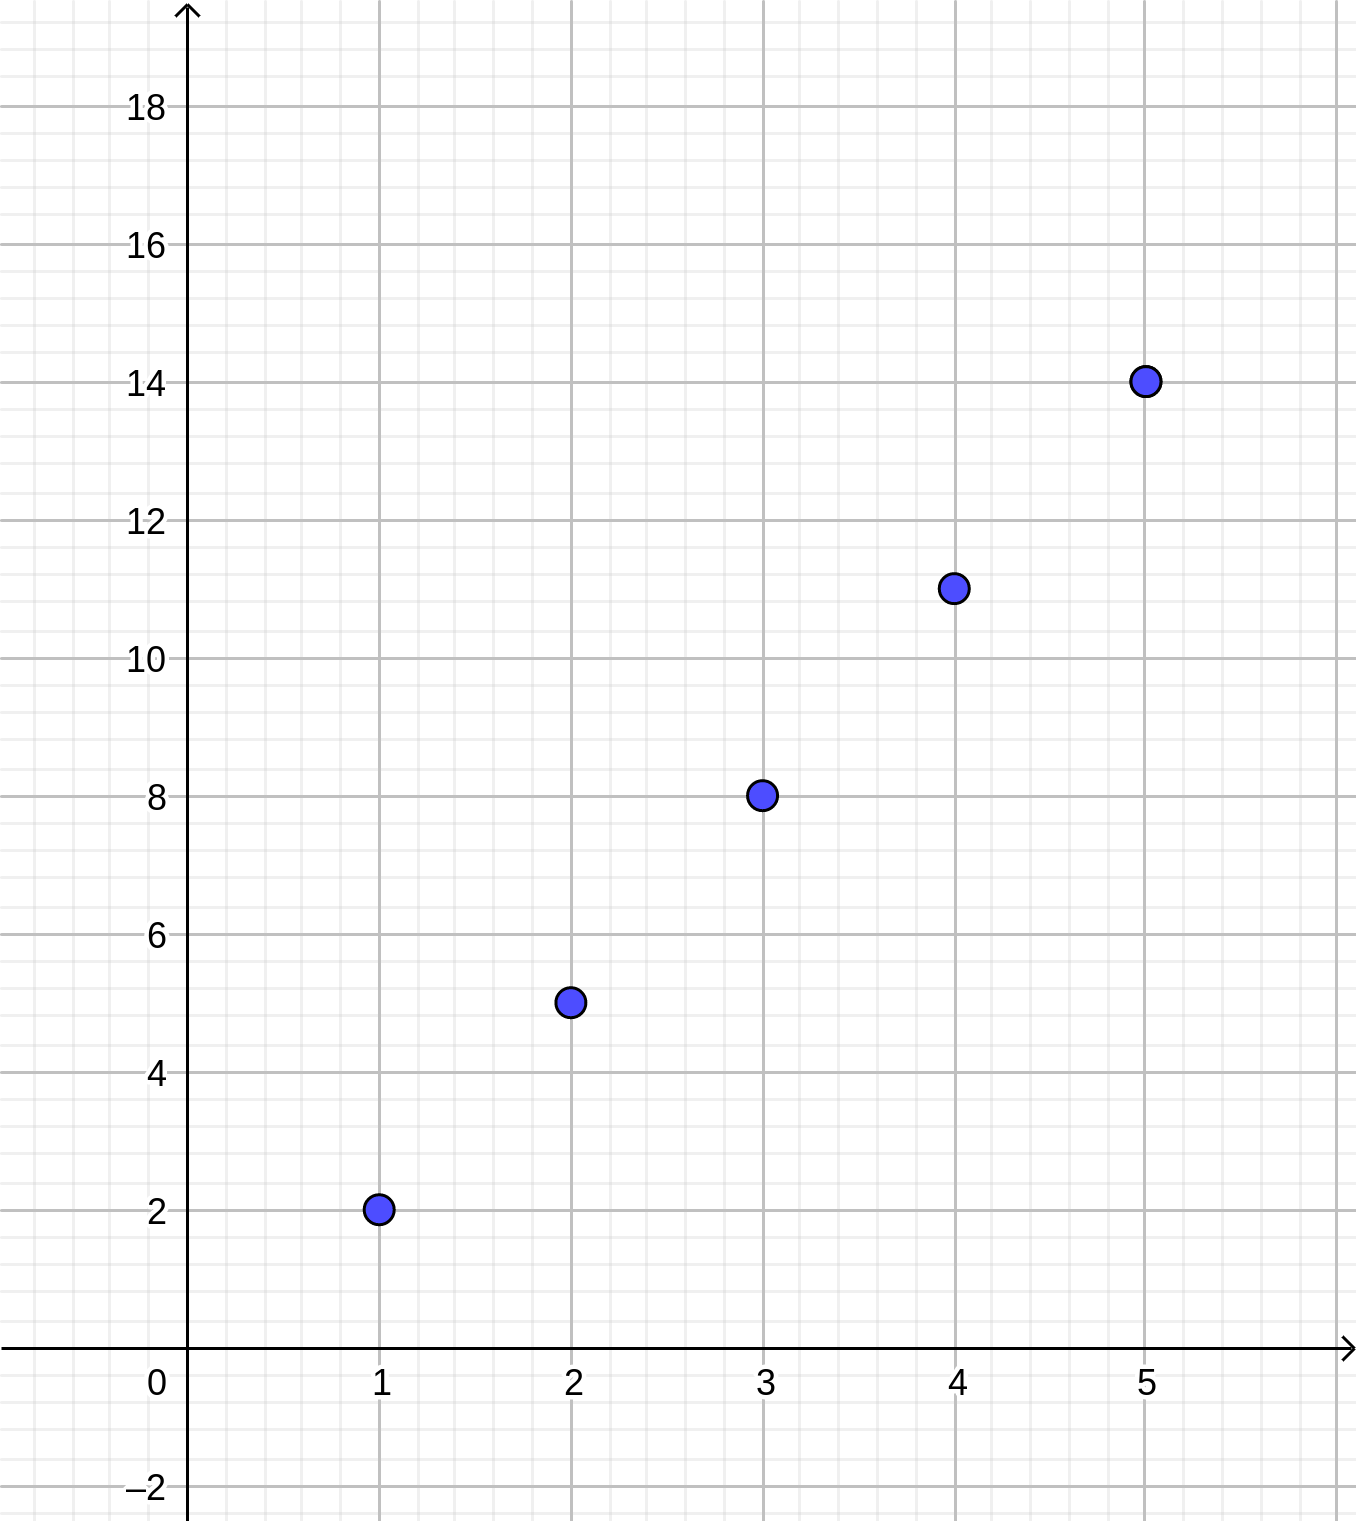
\includegraphics[height=8.4cm,keepaspectratio]{seqPlot}
\end{center}

\subsection{Exercise}
Plot on an appropriate set of axes the points corresponding to the sequences below:
\begin{enumerate}
	\item 3, 9, 15, 21, 27, ...
	\item 7, 9, 11, 13, 15, ...
	\item 10, 10.5, 11, 11.5, 12, ...
	\item 3, 1, -1, -3, -5, ...
	\item 0, 2, 4, 6, 8, ...
	\item 9, 10, 11, 12, 13, ...
	\item 8, 15, 22, 29, 36, ...
	\item 8, 1, -6, -13, -20, ...
	\item 8, 5.5, 3, 0.5, -2, ...
	\item 6, 6, 6, 6, 6, ...
	\item $n^{th}=2n+14$
	\item $n^{th}=5n-4$
	\item $n^{th}=8n+2$
	\item $n^{th}=2n-1$
	\item $n^{th}=3n+2$
	\item $n^{th}=-3n+20$
	\item $n^{th}=6n$
	\item $n^{th}=n^2$
	\item $n^{th}=7n-7$
	\item $n^{th}=-n$
\end{enumerate}

You can see that these points make a straight line if they are connected together.
\subsection{Special Sequences}
The special sequences that we are going to look at are: odd numbers, even numbers, square numbers and triangular numbers.  We will consider the numbers in their sequence and the formulae that produce them.

\subsubsection{Odd numbers}
The odd numbers go 1, 3, 5, 7, 9, ... . We can see that this is a linear sequence so that means that we know how to create a formula for it.  It goes up by 2 each time like the 2 times table, but all these values are 1 less, that implies that the formula is $n^{th}=2n-1$

\subsubsection{Even numbers}
The even numbers go 2, 4, 6, 8, ... . We can see that this is a linear sequence so that means that we know how to create a formula for it.  It goes up by 2 each time like the 2 times table, with no change, that implies that the formula is $n^{th}=2n$

\subsubsection{Square numbers}
Square numbers are calculated by counting the number of dots required to make a square.  So for example, if a square was 4 high and 4 wide we would need a total of 16 dots (4 rows of 4), this gives us the $4^{th}$ square number.  The first 5 square numbers in order are: 1, 4, 9, 16, 25.  The formula for finding square numbers is $n^{th}=n^2$

\subsubsection{Triangular numbers}
Triangular numbers are the number of dots that we get when we count the number of dots in a triangle.  Imagine a triangle with 1 dot at the top, 2 dots on the 2nd layer, 3 dots on the 3rd layer, 4 dots on the 4th layer and so on, these are the kind of triangles we are talking about.  So the 4th triangular number would come from a triangle with 4 layers, the number of dots would be $1+2+3+4=10$.  So the 4th triangular number is 10.

\subsection{Exercise}
With the following sequences compare them to the sequence of Square numbers and see if you can work out their formula would be:
\begin{enumerate}
	\item $2,5,10,17,26,37,...$
	\item $0,3,8,15,24,35,...$
	\item $11,14,19,26,35,46,...$
	\item $2,8,18,32,50,72,...$
\end{enumerate}
With the following sequences compare them to the sequence of Triangular numbers and see if you can work out their formula would be:
\begin{enumerate}
	\item $6,8,11,15,20,...$
	\item $0,2,5,9,14,...$
	\item $8,10,13,17,22,...$
	\item $2,6,12,20,30,...$
\end{enumerate}

\subsection{Solving for a sequence}
We are going to look at situations where we know the first part of the sequence.  From this we can work out the formula and then use the formula to work out which term has a particular value.

\begin{exmp}
If we have the sequence $5, 12, 19, 26, ...$ which term has the value 96?

First we want the formula for the sequence.  Our sequence goes up by 7 each time like the 7 times table, but each term is 2 less, so our formula is $n^{th}=7n-2$.

Now we know our particular nth term has a value of 96, so let's make the equation:

$7n-2=96$

If we solve this equation we get $n=14$, so it is the 14th term which equals 96.
\end{exmp}

\subsection{Exercise}
\begin{enumerate}
	\item For the sequence $4,10,16,22,...$ which term has the value $118$?
	\item For the sequence $9,13,17,21,...$ which term has the value $209$?
	\item For the sequence $27, 25, 23, 21, ...$ which term has the value $-117$?
	\item For the sequence $19,30,41,52,...$ which term has the value $481$?
\end{enumerate}

\subsection{Sequences in other situations}
When a given situation seems to follow a pattern we can often assign this to a sequence.

\begin{exmp}
Suppose a train engine is 10 m long and carridges are 7 m long. Train design 1 has 1 carridge and train design 2 has 2 carridges etc. Which train design is 59 m long.

First let's make a sequence for the different designs:

\bigskip

$17, 24, 31, 38...$

\bigskip

We can see that the formula for this sequence is $n^{th}=7n+10$ when $n$ is the design number and $n^{th}$ represents the length of the train.

\bigskip

So the equation we need to solve is $7n+10=59$ and the result is $n=7$.  So it is design 7 which is 59 m long.
\end{exmp}
\subsection{Exercise}
\begin{enumerate}
	\item A gardener buys a tree that is 1m tall and grows at a rate of 0.2m per year.  So at the end of the first year it is 1.2m tall.  Write a formula for how tall the tree will be after year 'n' and use this formula to work out the height of the tree after 11 years.
	\item A boy got a score of 17 on a maths test and decided to put in place a study program to improve.  The study program helped him improve his score by 3 each week, so that after 1 week he would get a score of 20.  Use a formula to calculate his score after 9 weeks and calculate after how many weeks it would be for him to get a score of 80.
	\item In my Youtube account I have 3478\cent \hspace{0.2cm} and I earn 87\cent \hspace{0.2cm} a day.  After how many days will it be for me to have a total of \$507?
	\item Rose was growing a rose. The flower grew 0.3 metres each week. It is 0.8 metres right now. How long will the flower be in 52 weeks? (1 year) (R.H.)
	\item Alice plants daisies.  In the first summer she planted 50 seeds and plants 17 more seeds in the each of the following summers.  How many seeds would she have planted in the first 15 years? (K.W.)
	\item Isobel decides to sail from New Zealand to Japan, she starts counting how many Kms she has travelled per day after she knows she has travelled 12km.  The next day she sees that she has now gone 21km.  If she continues at the same speed, how far will she have travelled after 11 days.  Also how far will she have travelled after 'n' days?  If it is 9346km to Japan how long will it take her to get there. (I.F.)
\end{enumerate}
\chapter{Measurement}
\section{Units}
In this chapter of the book we are interested in how we measure length, area and volume.  We will be using the metric system which is partly based on the metre.  This metre can be divided up or multiplied to give us units like mm, cm and km.  'Milli' means ${\frac{1}{1000}}^{th}$, 'centi' means ${\frac{1}{100}}^{th}$ and 'kilo' means 1000.

\bigskip

To change m to mm we multiply by 1000 since 'milli' means ${\frac{1}{1000}}^{th}$

To change m to cm we multiply by 100 since 'centi' means ${\frac{1}{100}}^{th}$

To change m to km we divide by 1000 since 'kilo' means 1000.

\begin{exmp}
Change 3.7m into cm.

\bigskip

To change m to cm we multiply by 100.

\bigskip

So $3.7m = (3.7 \times 100) cm = 370cm$
\end{exmp}

\begin{exmp}
Change 265m into km.

\bigskip

To change m to km we divide by 1000.

\bigskip

So $265m = (265 \div 1000)km = 0.265km$

\end{exmp}
\subsection{Exercise}
Change the following lengths in 'm' to the required unit:
\begin{enumerate}
	\item $4.7m$ to $cm$
	\item $5.34m$ to $mm$
	\item $65.7m$ to $cm$
	\item $3536m$ to $km$
	\item $46m$ to $km$
	\item $362m$ to $mm$
	\item $65.3m$ to $mm$
\end{enumerate}

\section{Perimeter}
The perimeter of a shape is the length around the outside or the total of the lengths of the sides.  So if I had a triangle with sides of lengths '3m', '5m' and '4.5m' the perimiter would be $(3+5+4.5)m = 12.5m$.
\subsection{Exercise}
Find the perimeter of the following shapes:
\begin{multicols}{2}
\begin{enumerate}
	\item 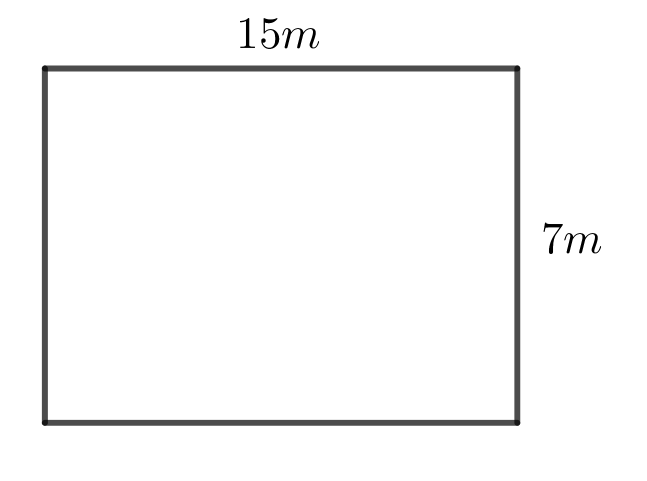
\includegraphics{./Images/Measurement/perimeter1.png}
	\item 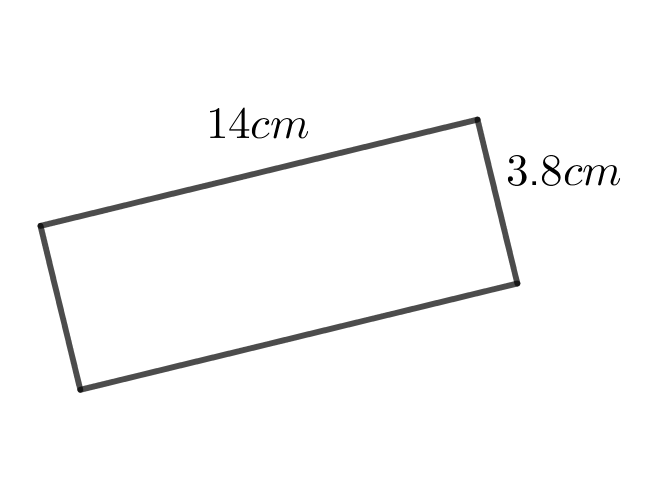
\includegraphics{./Images/Measurement/perimeter2.png}
	\item 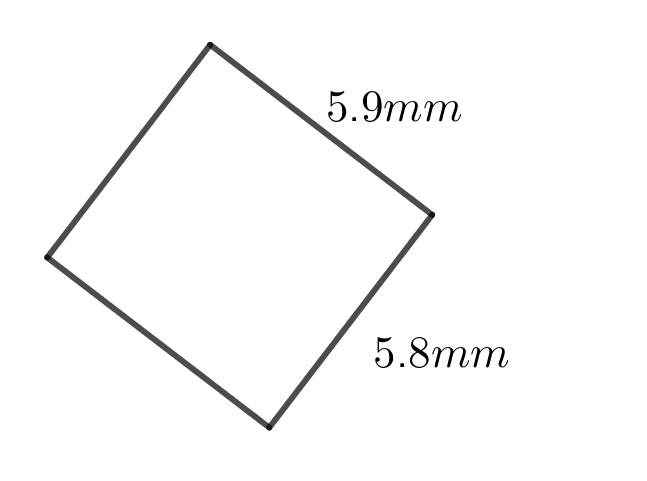
\includegraphics{./Images/Measurement/perimeter3.png}
	\item 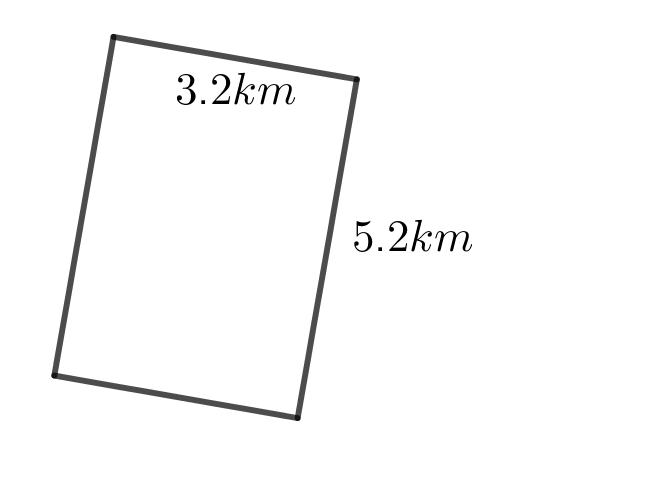
\includegraphics{./Images/Measurement/perimeter4.png}
	\item 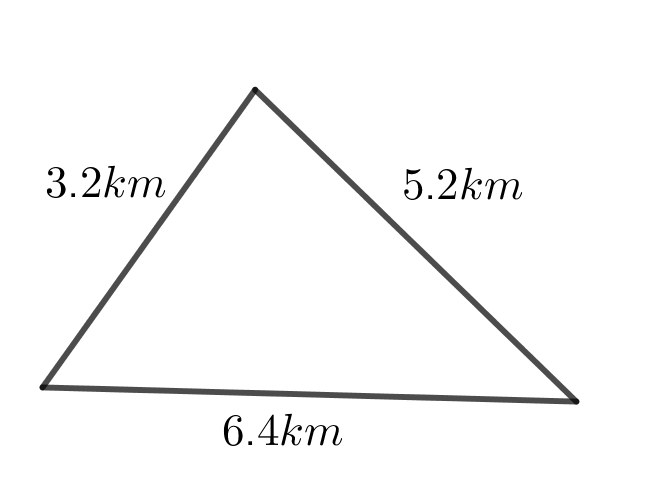
\includegraphics{./Images/Measurement/perimeter5.png}
	\item 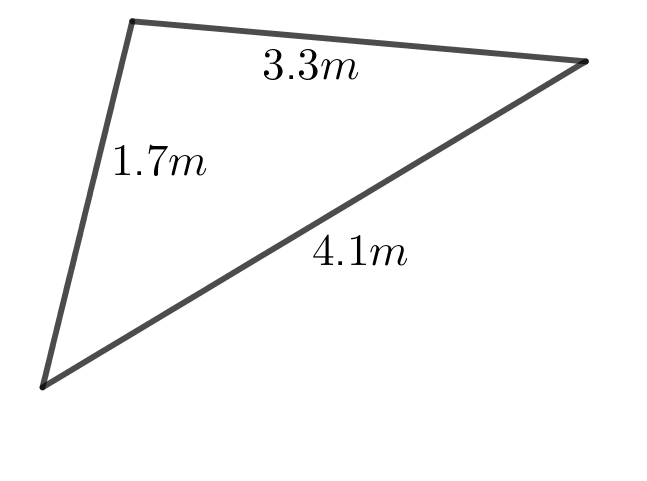
\includegraphics{./Images/Measurement/perimeter6.png}
	\item 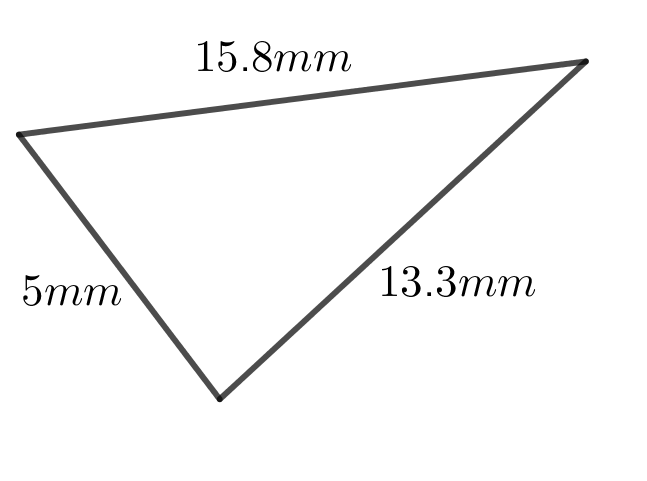
\includegraphics{./Images/Measurement/perimeter7.png}
	\item 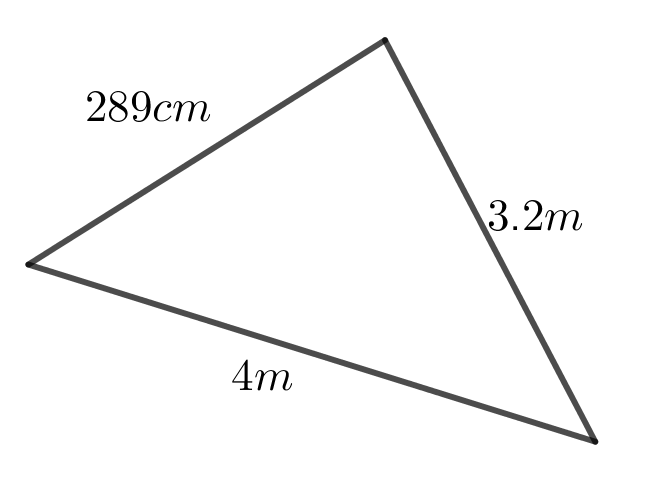
\includegraphics{./Images/Measurement/perimeter8.png}
	\item 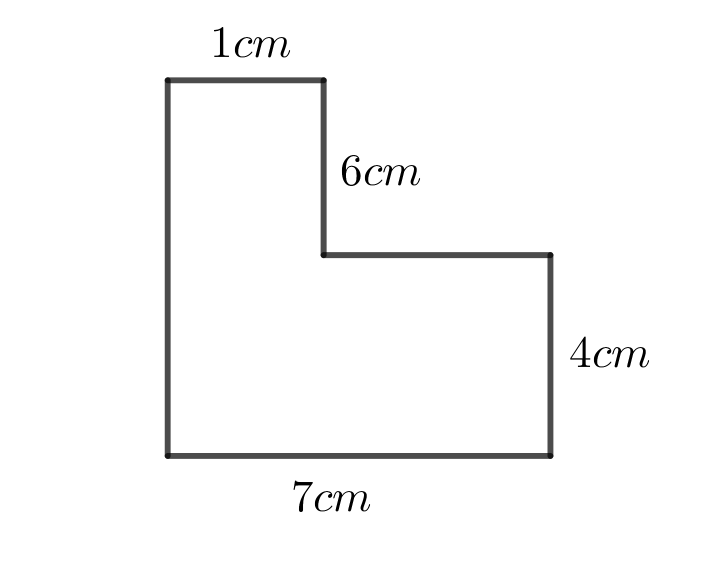
\includegraphics{./Images/Measurement/perimeter9.png}
	\item 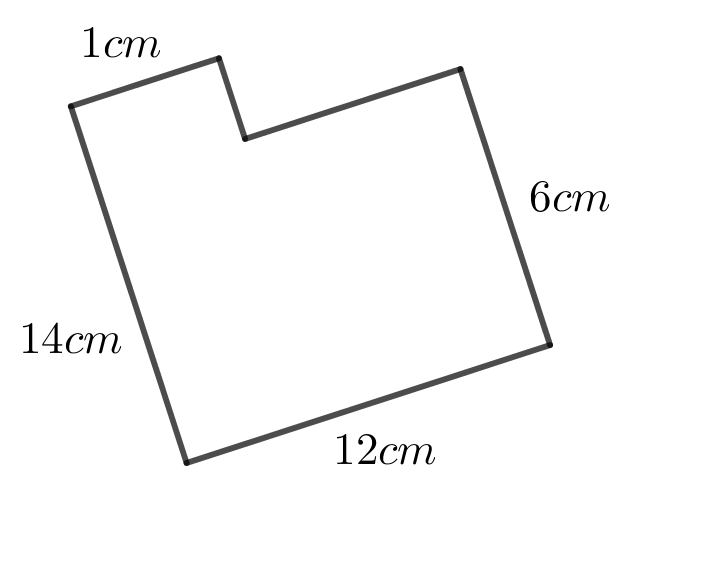
\includegraphics{./Images/Measurement/perimeter10.png}
	\item 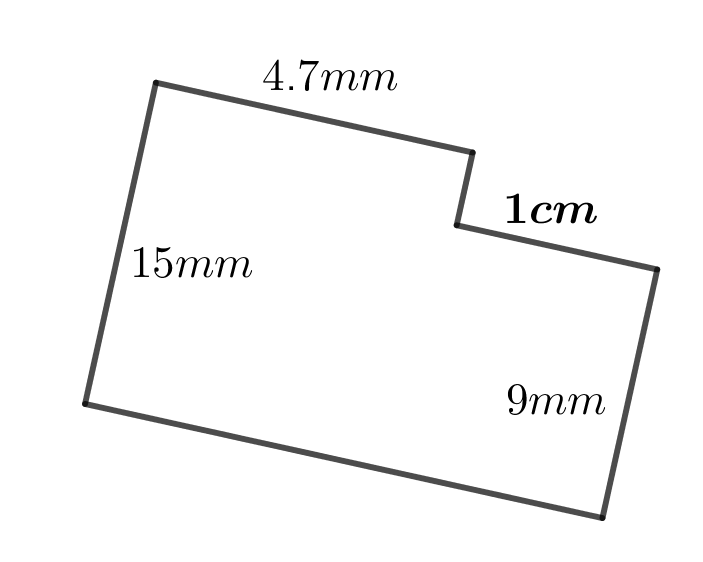
\includegraphics{./Images/Measurement/perimeter11.png}
	\item 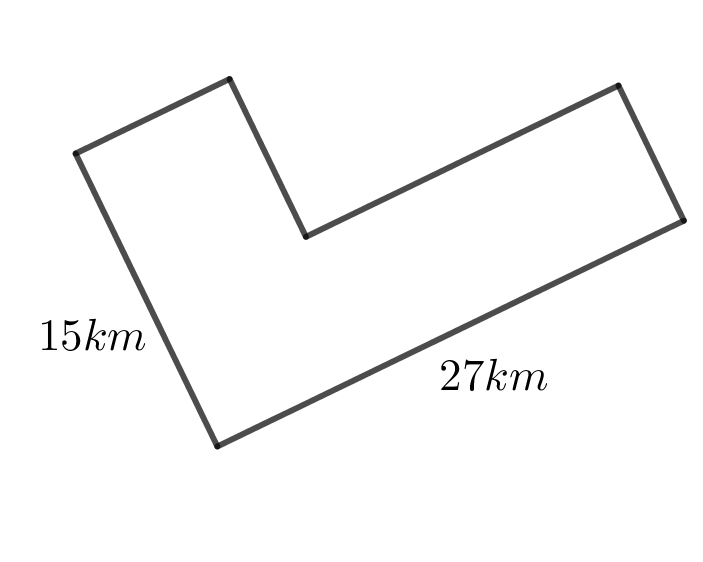
\includegraphics{./Images/Measurement/perimeter12.png}
\end{enumerate}
\end{multicols}
\subsection{Circles}
The perimeter of a circle is called the circumference.  The distance from one side of a circle to the other, through the centre, is called the diameter.  If we multiply the diameter by a particular value we can calculate the circumference.  Before I give you this value you might want to draw some circles and measure there diameters and circumferences and divide the circumference by the diameter.  When you have done that a few times continue reading.

\bigskip

If you did the exercise above, you should of got answers that were close to 3.  In fact if you managed to do it to 5 decimal places the value would have been $3.14159$.  This value is called $\pi$ which is called 'pi'.

\bigskip

To calculate the circumference of a circle we just use the formula $C=\pi d$

\begin{exmp}
Find the circumference of a circle that has a diameter of 15cm.

\bigskip

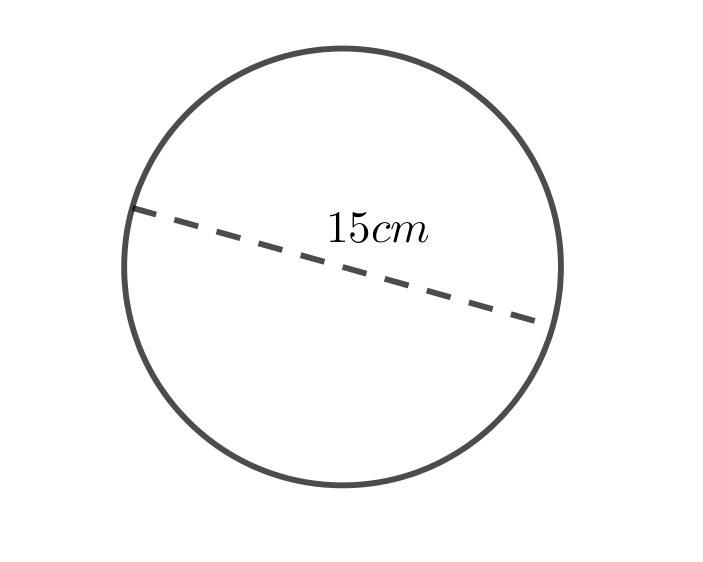
\includegraphics{./Images/Measurement/circumferenceEg1.png}

\bigskip

We know that $C=\pi d$, therefore the Circumference $=3.142 \times 15=47.13cm$
\end{exmp}

The radius of a cirle is the distance from the centre to the edge.  It follows that $C=2\pi r$
\begin{exmp}
Find the circumference of a circle that has a radius of 3.6km.

\bigskip

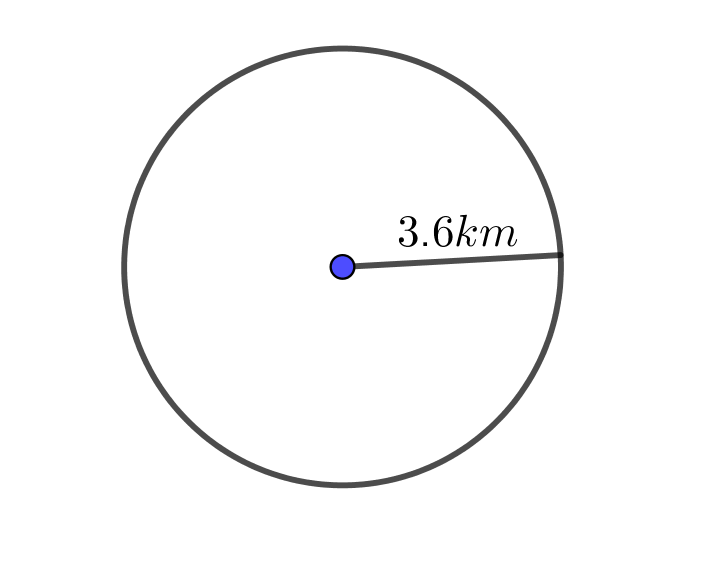
\includegraphics{./Images/Measurement/circumferenceEg2.png}

\bigskip

We know that $C=2\pi r$, therefore the Circumference $=2 \times 3.142 \times 3.6=22.622km$
\end{exmp}
\subsection{Exercise}
Find the circumference of the following circles:
\begin{enumerate}
	\item $d = 12km$
	\item $r = 6.34mm$
	\item $r = 18cm$
	\item $d = 78m$
	\item $d = 0.56mm$
	\item $r= 187km$
	\item $r = 35m$
	\item $d = 35.78m$
\end{enumerate}
\subsection{Algebraic}
\begin{exmp}
	Find $x$ given that the perimeter of the rectangle below is 58cm.

	\bigskip

	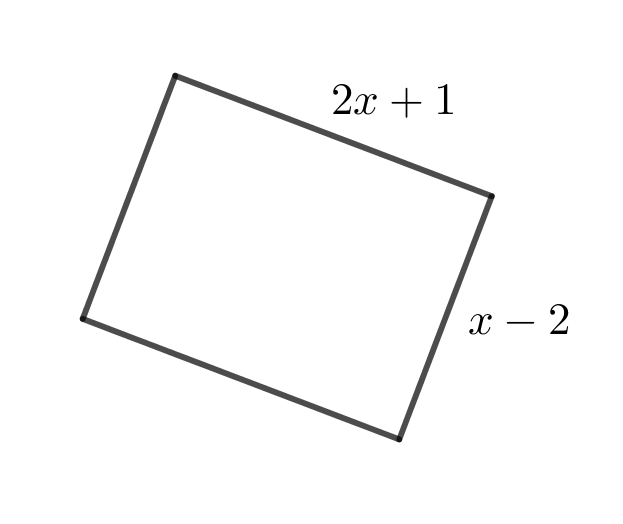
\includegraphics{./Images/Measurement/perAlgExmp1.png}

	\bigskip

	The perimeter of the shape is $2x+1+2x+1+x-2+x-2$

	\bigskip

	This simplifies to $6x-2$

	\bigskip

	Since we know the perimeter is also 58cm we can produce the equation $6x-2=58$

	\bigskip

	If we solve this equation we get $x = 10cm$

\end{exmp}

\subsection{Exercise}
Find the value of $x$ in the following:
\begin{multicols}{2}
\begin{enumerate}
	\item 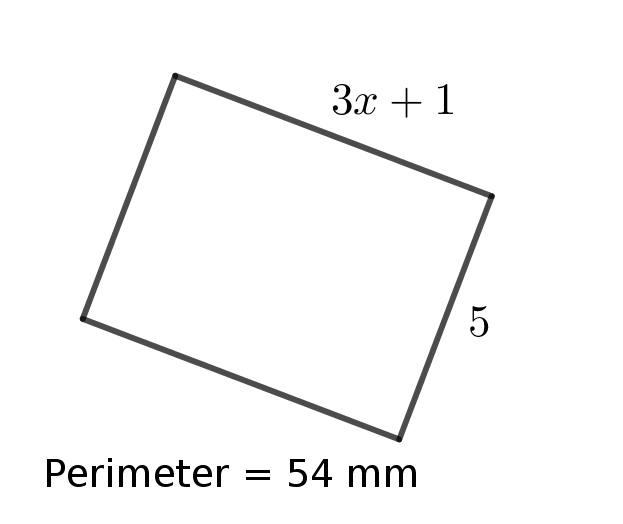
\includegraphics{./Images/Measurement/perAlg1.png}
	\item 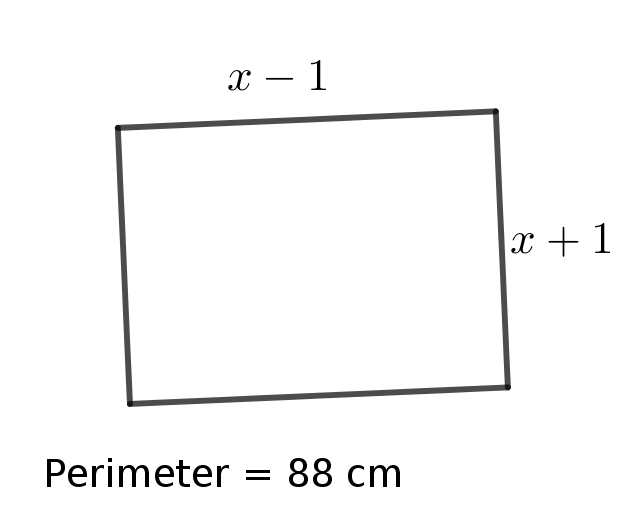
\includegraphics{./Images/Measurement/perAlg2.png}
	\item 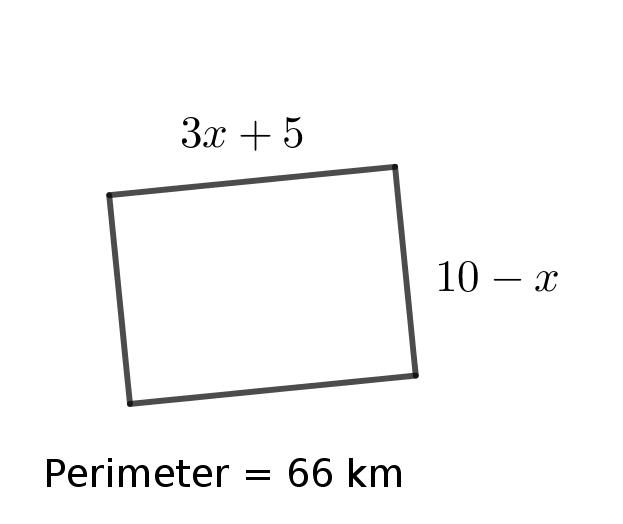
\includegraphics{./Images/Measurement/perAlg3.png}
	\item 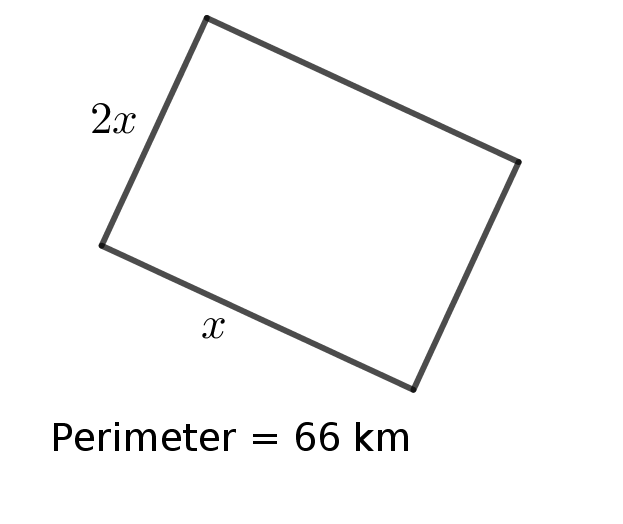
\includegraphics{./Images/Measurement/perAlg4.png}
	\item 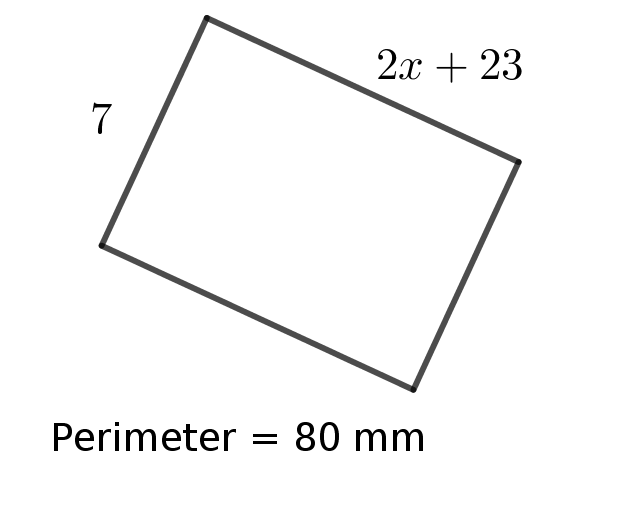
\includegraphics{./Images/Measurement/perAlg5.png}
	\item 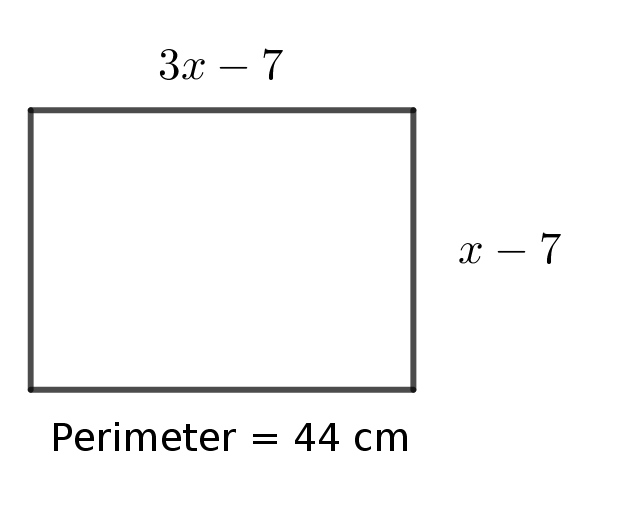
\includegraphics{./Images/Measurement/perAlg6.png}
\end{enumerate}
\end{multicols}
\section{Area}
The area of a shape is equal to the number of 1 by 1 squares that are required to cover it.

\subsubsection{Rectangle}
To calculate the area of a rectangle we multiply the length by the width.  This gives the formula:

\bigskip

$A=lw$

\begin{exmp}
	Find the area of a rectangle with a length of 7cm and a width of 10cm.

\bigskip

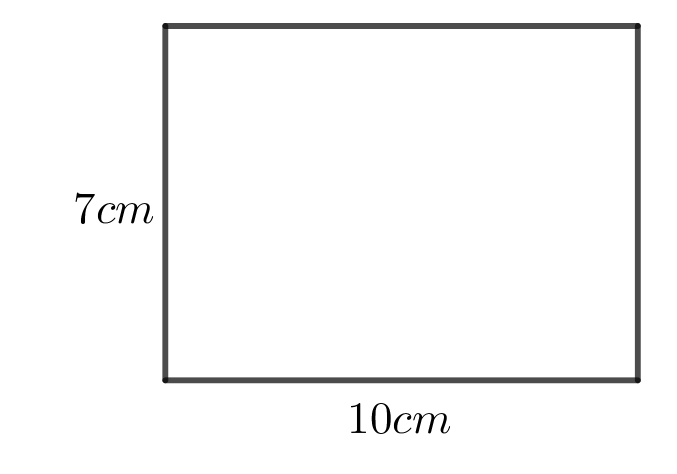
\includegraphics{./Images/Measurement/AreaEg1.png}

\bigskip

$A=lw$

\bigskip

So $A = 7 \times 10 = 70 cm^2$
\end{exmp}

\subsubsection{Triangle}
To calculate the area of a triangle we multiply the base length by the perpendicular height and divide by 2.  This gives the formula:

\bigskip

$A=\frac{bh}{2}$

\begin{exmp}
	Find the area of a triangle with a base length of 6mm and a height of 7mm.

\bigskip

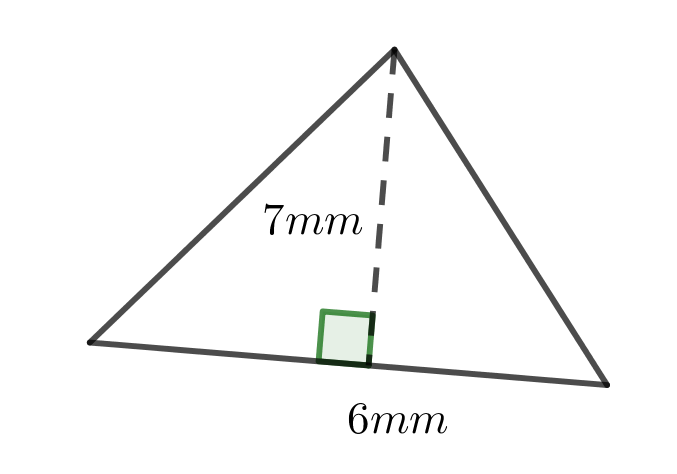
\includegraphics{./Images/Measurement/AreaEg2.png}

\bigskip

So $A = \frac{6 \times 7}{2} = 21 mm^2$
\end{exmp}
\subsubsection{Parallelogram}
To calculate the area of a parallelogram we multiply the base length by the perpendicular height.  This gives the formula:

\bigskip

$A=bh$

\begin{exmp}
	Find the area of a parallelogram which has a base length of 13 km and a perpendicular height of 5 km.

\bigskip

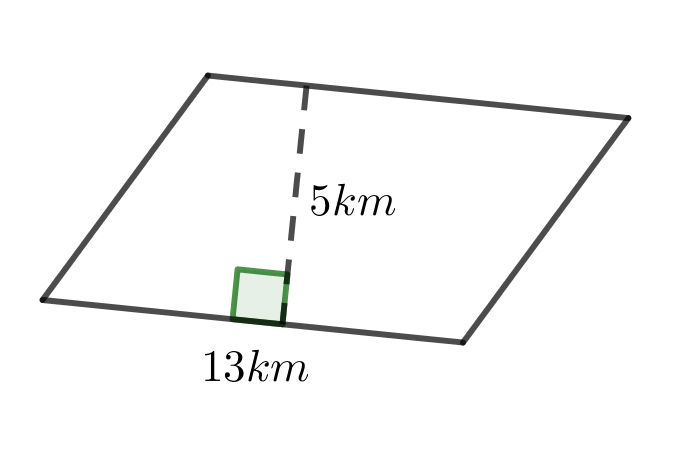
\includegraphics{./Images/Measurement/AreaEg3.png}

\bigskip

$A= 13 \times 5 = 65 km^2$
\end{exmp}

\subsubsection{Trapezium}
To calculate the area of a trapezium we multiply the average of the parallel sides by the perpendicular height (distance between them).  This gives the formula:

\bigskip

$A=\frac{(a+b)}{2}h$

\begin{exmp}
	Find the area of a trapezium which has paralell sides of lengths 6cm and 9cm and the distance between them is 8cm.

\bigskip

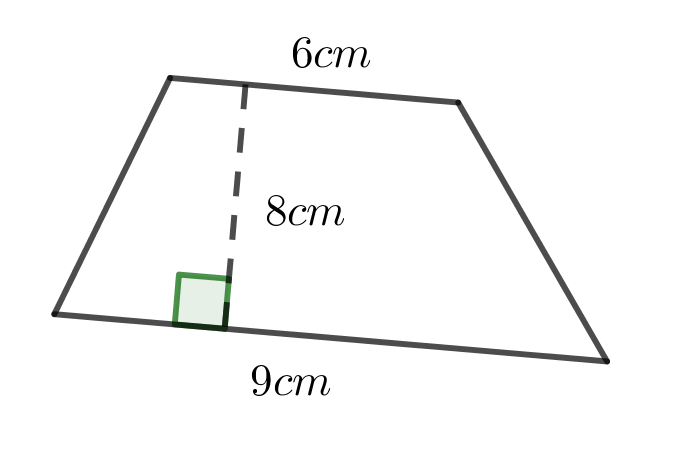
\includegraphics{./Images/Measurement/AreaEg4.png}

\bigskip

$A= \frac{(6+9)}{2}\times 8 = 60 cm^2 $
\end{exmp}

\subsection{Exercise}
Find the area of the following shapes.  Remember to show you working and include the correct units.
\begin{multicols}{2}
\begin{enumerate}
	\item 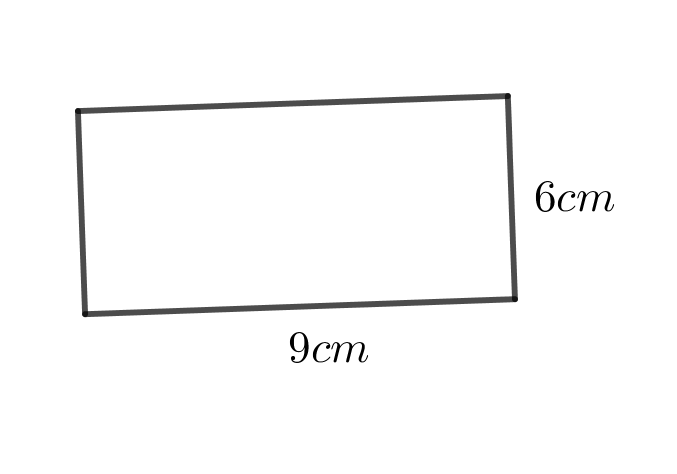
\includegraphics{./Images/Measurement/AreaQu1.png}
	\item 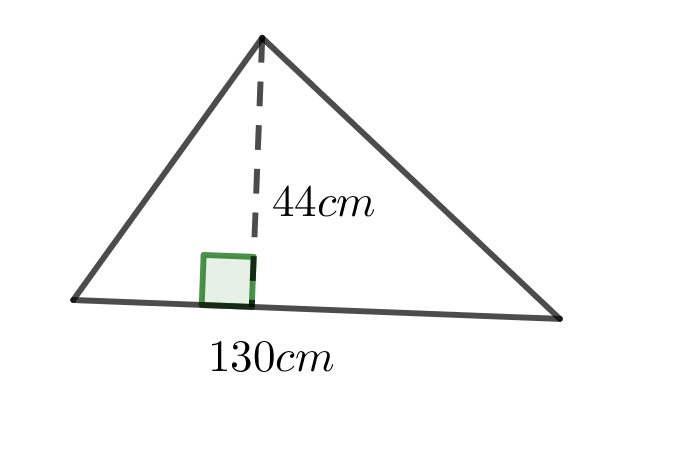
\includegraphics{./Images/Measurement/AreaQu2.png}
	\item 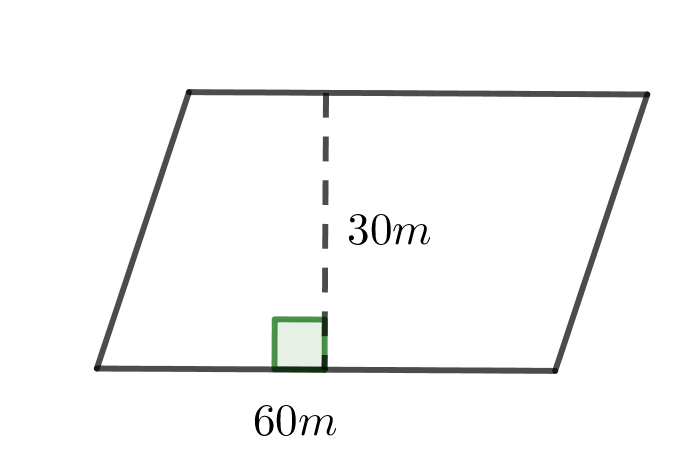
\includegraphics{./Images/Measurement/AreaQu3.png}
	\item 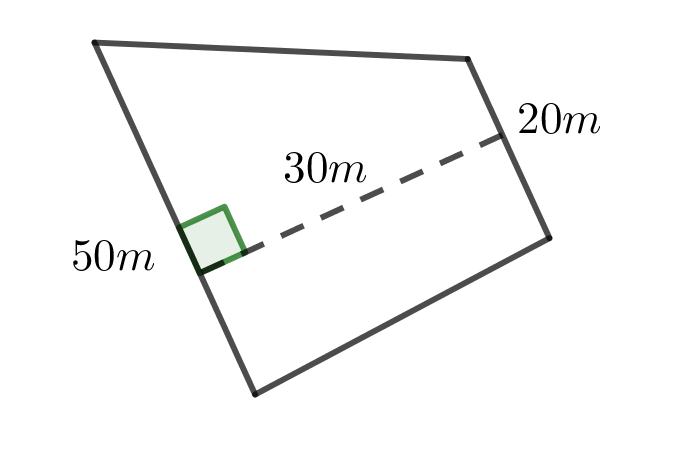
\includegraphics{./Images/Measurement/AreaQu4.png}
	\item 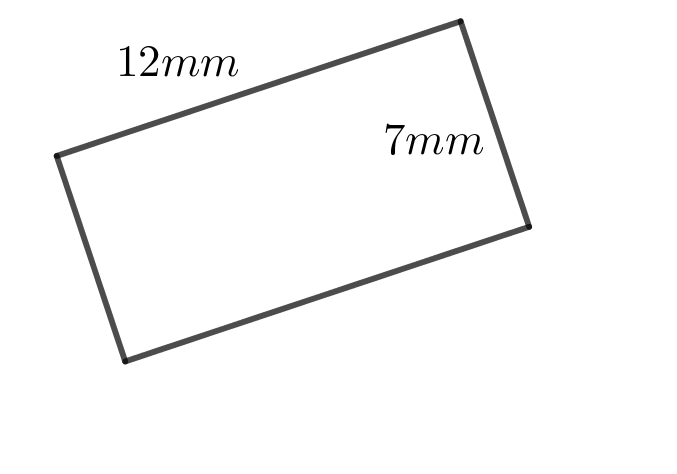
\includegraphics{./Images/Measurement/AreaQu5.png}
	\item 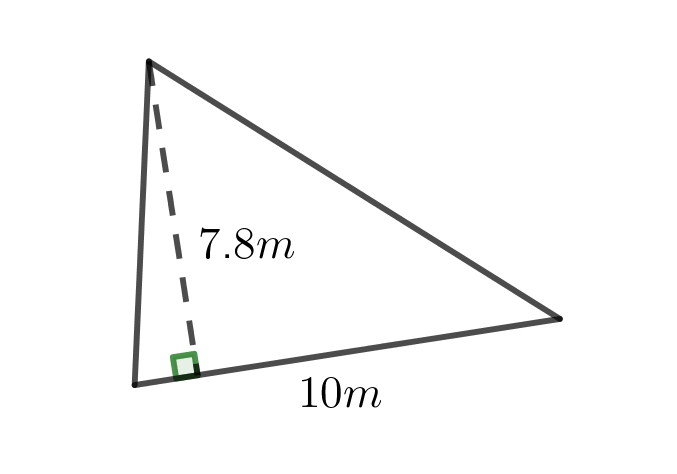
\includegraphics{./Images/Measurement/AreaQu6.png}
	\item 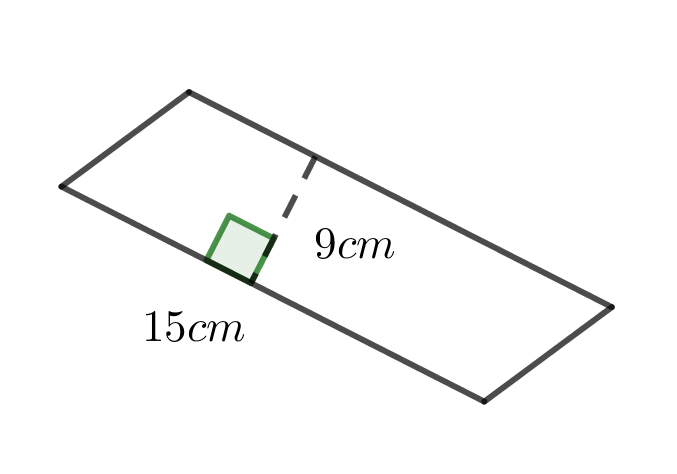
\includegraphics{./Images/Measurement/AreaQu7.png}
	\item 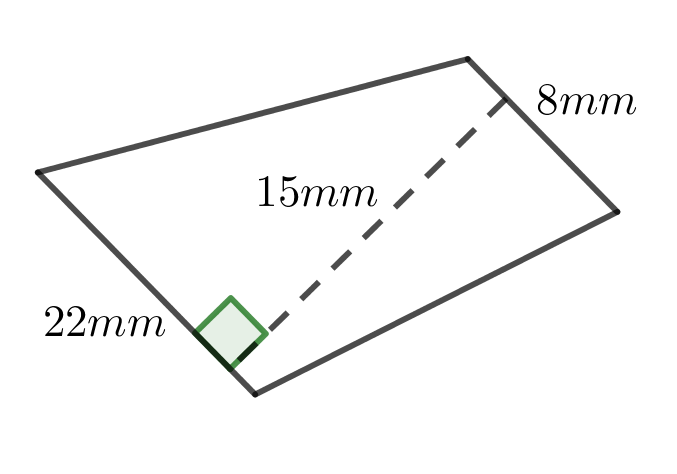
\includegraphics{./Images/Measurement/AreaQu8.png}
	\item 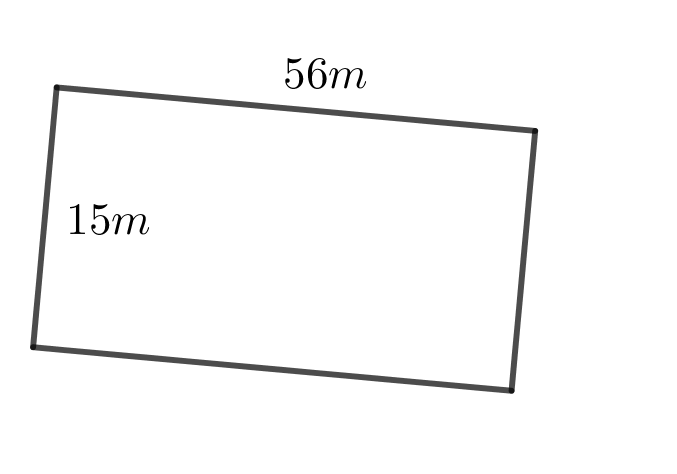
\includegraphics{./Images/Measurement/AreaQu9.png}
	\item 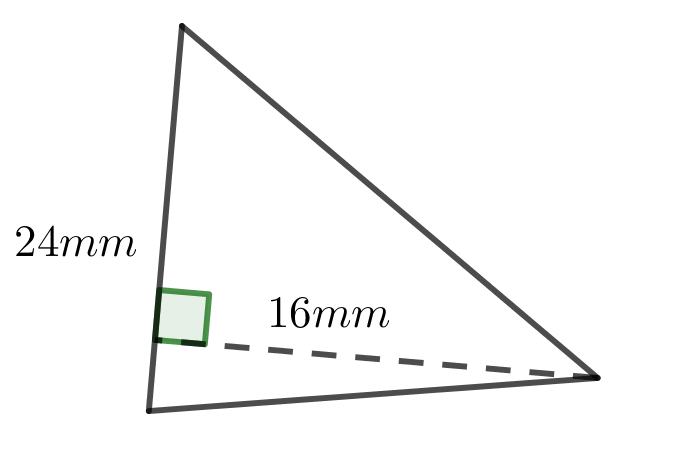
\includegraphics{./Images/Measurement/AreaQu10.png}
	\item 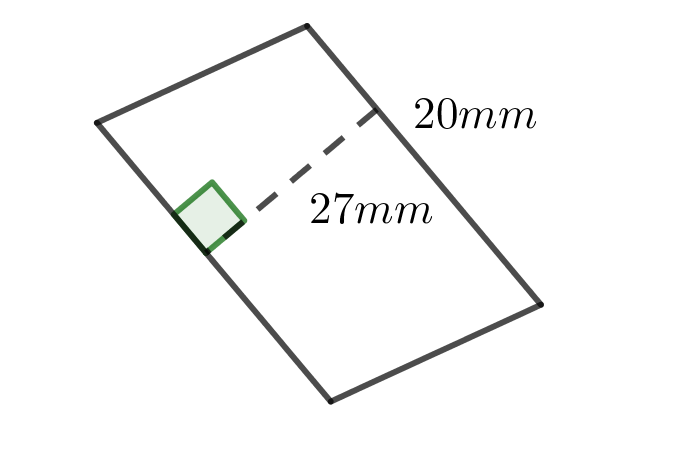
\includegraphics{./Images/Measurement/AreaQu11.png}
	\item 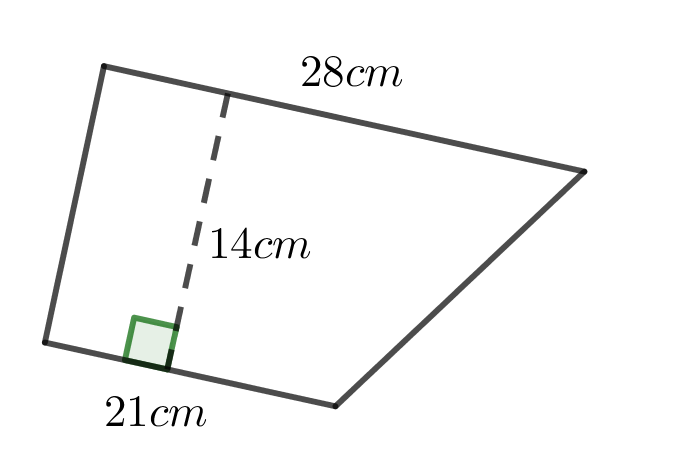
\includegraphics{./Images/Measurement/AreaQu12.png}
	\item 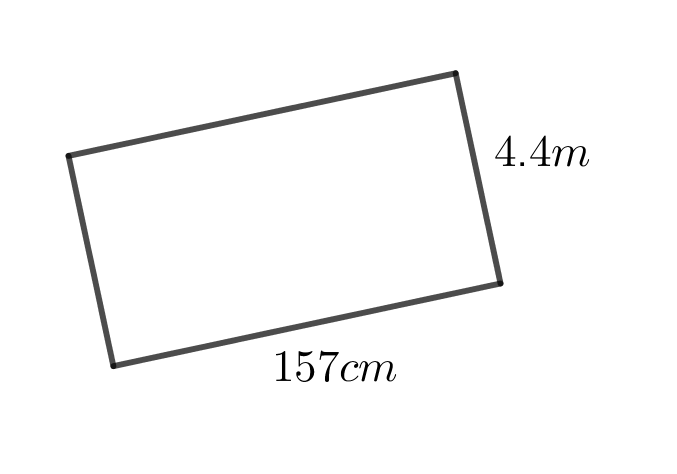
\includegraphics{./Images/Measurement/AreaQu13.png}
	\item 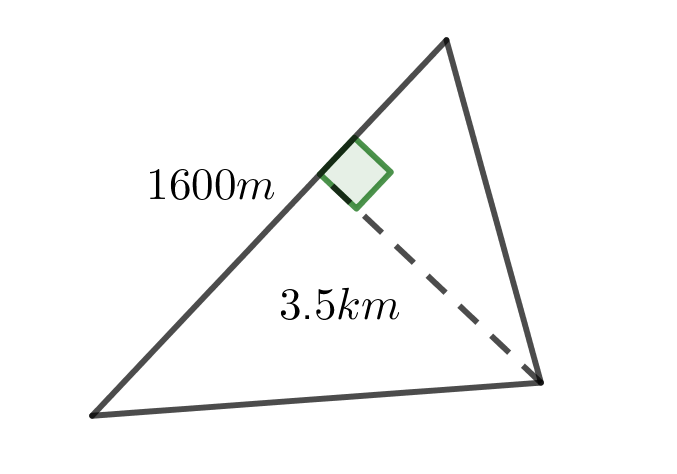
\includegraphics{./Images/Measurement/AreaQu14.png}
	\item 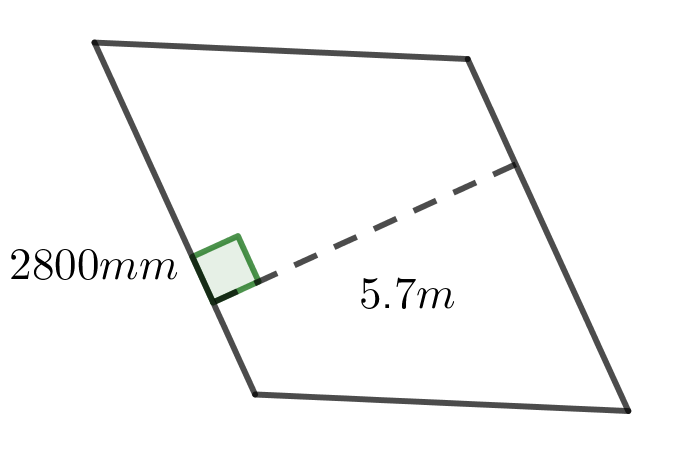
\includegraphics{./Images/Measurement/AreaQu15.png}
	\item 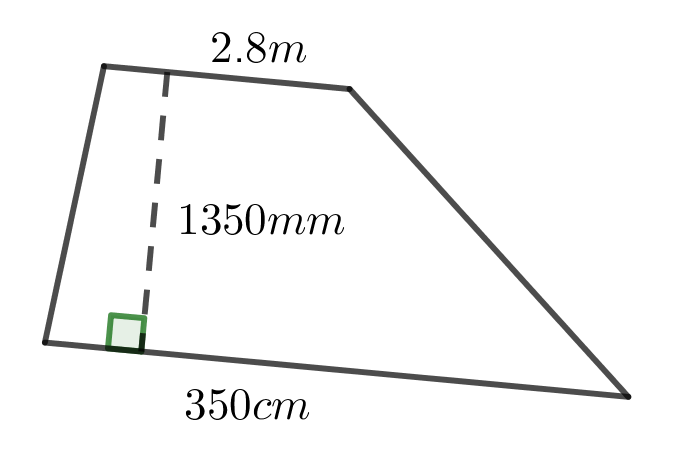
\includegraphics{./Images/Measurement/AreaQu16.png}
\end{enumerate}
\end{multicols}
\subsection{Circles}
Imagine a  circle with a radius 'r', split into sectors.

\bigskip

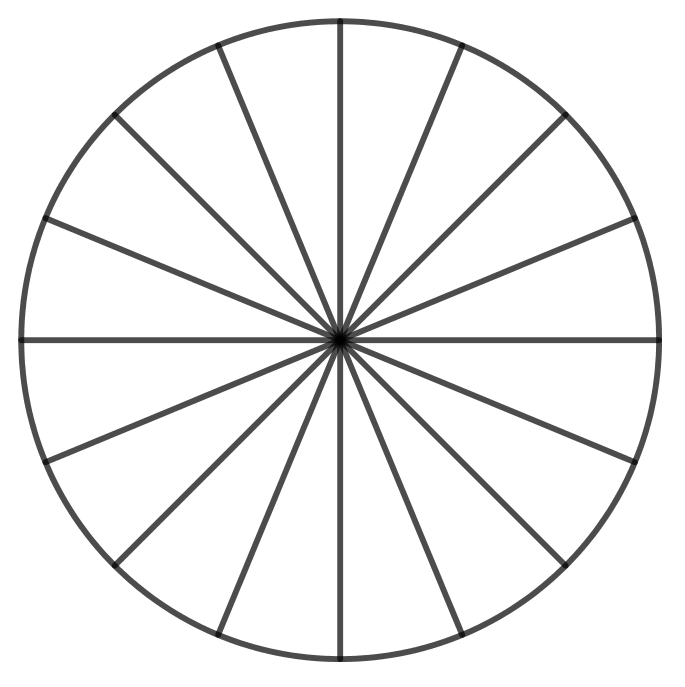
\includegraphics{./Images/Measurement/CircleSegmented.png}

\bigskip

Now rearrange the sectors as below

\bigskip

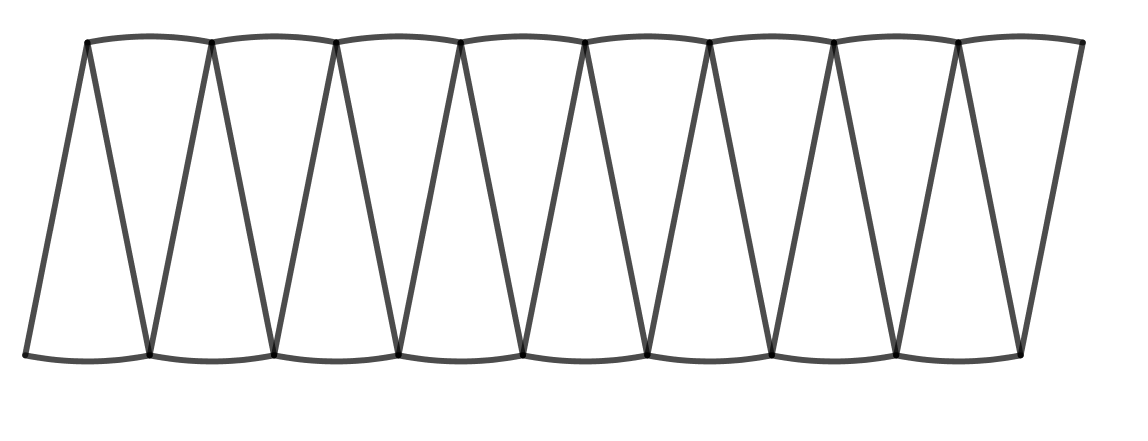
\includegraphics{./Images/Measurement/Circle2Rec.png}

The more sectors that we split our circle into the closer our rearranged shape becomes like a rectangle.  We can clearly see that this rectangle will have a height of 'r', but what is its length.  We can see that the two lengths are made up of the circumfernce of the circle which we know is $2 \pi r$, so one length would be just $\pi r$.

The area of this rectangle then would be $r \times \pi r = \pi r^2$

\bigskip

The area of a circle is found using $A=\pi r^2$

\begin{exmp}
Find the area of a circle with a radius of 5m.

\bigskip

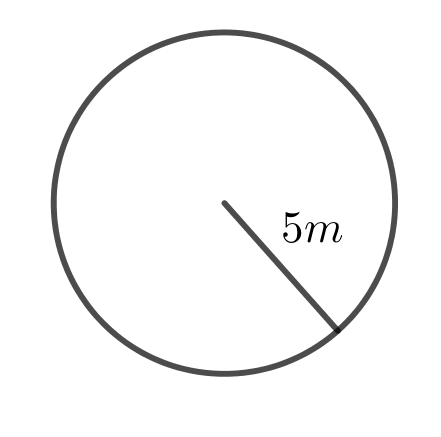
\includegraphics{./Images/Measurement/CircleAreaEg1.png}

\bigskip

So $A = \pi r^2 = \pi \times 5^2 = 78.54 m^2$


\end{exmp}

\begin{exmp}
Find the area of a circle with a diameter of 8.6mm.

\bigskip

\includegraphics{./Images/Measurement/CircleAreaEg2.png}

\bigskip

The radius is half the diameter so the radius is 4.3mm.

\bigskip

So $A = \pi r^2 = \pi \times 4.3^2 = 58.1 mm^2$

\end{exmp}

\subsection{Exercise}
Find the areas of the following circles, make sure you include the units.
\begin{multicols}{2}
\begin{enumerate}
	\item \includegraphics{./Images/Measurement/CircleAreaEx1.png}
	\item \includegraphics{./Images/Measurement/CircleAreaEx2.png}
	\item \includegraphics{./Images/Measurement/CircleAreaEx3.png}
	\item \includegraphics{./Images/Measurement/CircleAreaEx4.png}
	\item \includegraphics{./Images/Measurement/CircleAreaEx5.png}
	\item \includegraphics{./Images/Measurement/CircleAreaEx6.png}
\end{enumerate}
\end{multicols}

\subsection{Surface Area}
The surface area of a shape is equal to the total of the areas of it various surfaces.  Normally we would work this out by sketching each of the surfaces as if they were flat, work out their individual areas and then add them.  We will look at the special cases of cuboids, cylinders and spheres and then look at some examples of 'odd' shapes.
\subsubsection{Cuboids}
A cuboid is like a box.

\bigskip

\includegraphics{./Images/Measurement/CuboidPic.png}

\bigskip

Opposite faces are identical, so it is made up three pairs of faces.

If we have a cuboid which is $l \times w \times h$ then the three faces will be:

\begin{itemize}
	\item $l \times w$
	\item $l \times h$
	\item $w \times h$
\end{itemize}

We can work each of these areas out add them together and multiply the answer by 2.

\begin{exmp}
Find the surface area of the cuboid below:

\bigskip

\includegraphics{./Images/Measurement/CuboidEg.png}

\bigskip

First we change the lengths all to the same unit, I will choose $m$.  So we have a $2m \times 1.2m \times 0.85m$ cuboid.

The three faces are:

\begin{itemize}
	\item $2 \times 1.2 = 2.4m^2$
	\item $2 \times 0.85 = 1.7m^2$
	\item $1.2 \times 0.85 \approx 1m^2$
\end{itemize}

The surface area is $2 \times (2.4 + 1.7 + 1)=10.2m^2$
\end{exmp}

\subsubsection{Cylinder}
A cylinder is made up of two identical circls joined by a curved rectangle.

\bigskip

\includegraphics{./Images/Measurement/CylinderNet.png}

\bigskip

To calculate the area of the circles we need their radius to work out the area of the rectangle we need the rectangles height and width.  Since the rectangle is curved around the circles its width must equal the circumference of the circle, so we can use $2 \pi r$ to obtain the width of the rectangle.

\begin{exmp}
Find the surface area of the cylinder below:

\bigskip

\includegraphics{./Images/Measurement/CylinderEg.png}

\bigskip

The circles have a radius of $4cm$, so the area of each circle is $\pi \times 4^2 = 50.27cm^2$

The circumference of a circle is $2 \times \pi \times 4 = 25.13cm$, so the area of the rectangle is $25.13 \times 7 = 175.9cm^2$

Therefore the surface area is $2 \times 50.27 + 175.9 = 276.5cm^2$

\end{exmp}


\subsubsection{Sphere}
The surface area of a sphere is calculated with the formula $A = 4 \pi r^2$

\begin{exmp}
Find the surface area of a sphere with a diameter of $10cm$.

The radius is $5cm$, so the surface area is $4 \times \pi \times 5^2=314cm^2$
\end{exmp}

\subsubsection{Odd shapes}
Here we find teh area of each face no matter what shape it is and add the values together.

\begin{exmp}
Find the surface area of the shape below:

\bigskip

\includegraphics{./Images/Measurement/OddSA.png}

\bigskip

We have a total of 8 faces (6 rectangles and 2 'L' shapes)

Three of the rectangles have areas of $1 \times 5 = 5cm^2$
Two of the rectangles have areas of $2 \times 5 = 10cm^2$
One  of the rectangles have areas of $3 \times 5 = 15cm^2$
The two 'L' shapes have areas of $4cm^2$

That gives a total surface area of $58cm^2$
\end{exmp}
\subsection{Exercise}
Find the surface area of the following shapes:

\subsection{Expanding Brackets}
When we talk about expanding brackets we mean multiplying a bracket by a a term or another bracket.  We can get questions in the form:

Expand $5(x+7)$  or $(x-4)(x+6)$

We are going to use the areas of rectangles to show how this works.

Let's consider $4(3+4)$.  We can see quite easily that the answer to this is 28 using BEDMAS.  Now let's look at the rectangle that represents this situation.

\bigskip

\includegraphics{./Images/Measurement/ExpandBrackets1.png}

\bigskip

The area of A is 12 and the area of B is 16, so the total is 28.  It should be noted that we did this by multiplying the 4 by 3 and the 4 by 4.

\bigskip

Now let's consider $x(x+6)$

\bigskip

\includegraphics{./Images/Measurement/ExpandBrackets2.png}

\bigskip

Here area A is $x^2$

\bigskip

The area of B is $6x$

\bigskip

So the total area is $x^2+6x$.  We got this by multiplying the $x$ by both terms in the bracket.

\bigskip

Now let's consider $x(x-3)$

\bigskip

\includegraphics{./Images/Measurement/ExpandBrackets3.png}

\bigskip

Rectangle A has a length of $x-3$ and a height of $x$ so this is the area we require.

\bigskip

The total area is $x^2$, the area of B is $3x$

\bigskip

So the required area is $x^2 - 3x$.  Again we multiplied the $x$ on the outside with all the terms within the bracket.

\bigskip

Finally, let's consider $(x+5)(x+3)$

\bigskip

\includegraphics{./Images/Measurement/ExpandBrackets4.png}

\bigskip

The area of A is $x^2$, the area of B is $3x$, the area of C is $5x$ and the area of D is $15$

\bigskip

So the total area is $x^2 + 8x + 15$ which is the expansion of $(x+5)(x+3)$

\begin{exmp}
Expand $(x+2)(2x-5)$

\bigskip

We multiply each term in the first bracket by each term in the second bracket.

\bigskip

$(x+2)(2x-5)=2x^2-5x+2x-10$

So $(x+2)(2x-5)=2x^2-3x-10$
\end{exmp}

\subsection{Exercise}
Expand and simplify each of the expressions below:
\begin{multicols}{3}
\begin{enumerate}
	\item $4(x+7)$
	\item $9(6-x)$
	\item $x(x+5)$
	\item $4(x+y)$
	\item $x(x-y)$
	\item $x(x+y+z)$
	\item $3x(x+2)$
	\item $5x(3x-4)$
	\item $(x+2)(x+5)$
	\item $(p+7)(p+4)$
	\item $(t+4)(t+3)$
	\item $(d+5)(d+6)$
	\item $(x+5(x-4)$
	\item $(y-6)(y+3)$
	\item $(t+2)(t-2)$
	\item $(g+10)(g-10)$
	\item $(2x+4)(x+7)$
	\item $(3x-7)(2x+4$
	\item $(5x-3)(x-5)$
	\item $(3t-5)(3t+1)$
	\item $(t-4)^2$
	\item $(4-t)^2$
	\item $(2x+3)^2$
	\item $(x+y)^2$
\end{enumerate}
\end{multicols}

\section{Volume}
When we are finding the volume of a shape we are calculating the number of unit cubes that will fit in it.

\chapter{Algebra 4}
\section{Exponents}
Just like multiplication is a short hand for repeated addition, exponnents are a short hand for repeated multiplication.  The exponent tells us how many times the value has been multiplied by itself and only applies to the value immediately to its left.

\bigskip

So $5^3$ means $5 \times 5 \times 5$ 

\bigskip

and $4x^2$ means $4 \times x \times x$

\subsection{Exercise}
Exand the following expressions and if possible find the value:
\begin{enumerate}
	\item $4^3$
	\item $2^5$
	\item $x^3$
	\item $2^3 + 3^2$
	\item $y^4$
	\item $5 \times 3^2$
\end{enumerate}

\subsection{Exercise}
Write the following expressions with exponents:
\begin{enumerate}
	\item $4 \times 4 \times 4 \times 4 \times 4 \times 4$
	\item $x \times x \times x \times x$
	\item $5 \times y \times y$
	\item $a \times b \times b \times b$
	\item $2 \times 5 \times t \times t \times m$
	\item $a \times b \times a \times a \times b$
\end{enumerate}

\section{Like Terms}
The number at the front of a term is called a coefficient and the rest of the term tells us its type.  The coefficient tells us how many of a particular type we have.  For two terms to be the same the parts after the coefficient must be identical.

\begin{exmp}
$3x+4x$, since both are of type $x$, they can be joined to become $7x$
\end{exmp}
\begin{exmp}
$4x + 7y$, one is of type $x$ and one is of type $y$ so they can't be joined so it remains as $4x+7y$
\end{exmp}
\begin{exmp}
$5x^2 - 3x + 4x$, we clearly have two $x$ terms so this can be simplified to $5x^2+x$.  Now these are two different types, one $x^2$ and the other $x$, so the expressions stays as $5x^2+x$
\end{exmp}
\begin{exmp}
$8x^2y - 6xy^2$, one of these is of type $x^2y$ and the other is of type $xy^2$.  They are different so the expression does not change.
\end{exmp}
\begin{exmp}
$xy + yx$, the order is different, but these are both of type $xy$, so can be simplified to $2xy$
\end{exmp}

\subsection{Exercise}
Where possible simplify the expressions below:
\begin{enumerate}
	\item $5x+7x$
	\item $6x+4y + 3x$
	\item $4xy - 2x + y$
	\item $5x^2-3x^2+6xy+2xy$
	\item $4pq-3qp$
	\item $5x^2+4x^2+7$
	\item $6st+3s-4st+5t$
	\item $4x+5x$
	\item $6h+3h+7h$
	\item $9t-t$
	\item $5+6g-2g+7$
	\item $4-5k-3k$
	\item $3x+5x+6y-2y$
	\item $7x+3y-2x-3y$
	\item $4x^2+5x-x^2+7$
	\item $3+5xy+2x-3y+5x+8$
	\item $6x^2+3x-5x+8$
	\item $4x^2+8xy-3xy+2y^2$
	\item $5x^3-4xy+y^2-3x^2+4y^2$
	\item $4a^2b+3ab^2$
	\item $6f^2+f5-4f-5f^2$
\end{enumerate}
\section{Dimensional Analysis}
\section{Solving Linear Equations}
We have already learnt how to solve questions of the form $ax+b=c$, we are now going to learn how to solve all linear equations.

\bigskip

Let's consider equations of the form $ax+b=cx+d$.  Often in mathematics when we are trying to solve a complex problem we just try and change it to a simplier problem that we can solve, that is what we are going to do here.  So we are going to change our problem into the form $ax+b=c$, we will do this by subtracting the value of the smallest $x$ term from both sides of the equation.

\begin{exmp}
Solve the equation $5x-7=3x+13$

\bigskip

The smallest $x$ term is $3x$ so we will subtract $3x$ from both sides of the equation.

\bigskip

So we now have $2x-7=13$

\bigskip

Now $+7$ to both sides.

\bigskip

We now have $2x=20$

\bigskip

So $x=10$
\end{exmp}

\begin{exmp}
Solve the equation $2x+5=17-4x$

\bigskip

The smallest $x$ term here is not $2x$, but $-4x$ since it is negative.  So we must subtract $-4x$ from both sides so that means we must $+4x$ to both sides of the equation.

\bigskip

So we now have $6x+5=17$

\bigskip

Now we $-5$ from both sides of the equation.

\bigskip

So we have $6x=12$

\bigskip

So $x=2$
\end{exmp}

\subsection{Exercise}
Find the value of $x$ in each of the equations.
\begin{multicols}{2}
\begin{enumerate}
	\item $5x-8=x+20$
	\item $6x+4=3x+13$
	\item $3x-5=27-5x$
	\item $5x+6=3x+10$
	\item $7x-5=4x+20$
	\item $4x+6=3x+20$
	\item $5x-8=x+4$
	\item $3x+6=8x-4$
	\item $2x-6=5x-24$
	\item $3x-9=10x-58$
	\item $2x-8=4-2x$
	\item $2x-5=7-x$
	\item $6-3x=10-5x$
	\item $5x+2=x+14$
	\item $2-3x=14-7x$
	\item $8x-5=4x+7$
	\item $8-2x=2x-4$
	\item $4x+7=9x-3$
\end{enumerate}
\end{multicols}
\subsection{Brackets}
When we have equations that contain brackets it is often best, but not always, to expand the brackets first, this will usually leave us with a problem like the previous ones.  A more complicated situation might require us to group like terms.  We will look at two examples one where the bracket gets multiplied by a positive value and one where we multiply by a negative value.

\begin{exmp}
Solve the equation $3(x+4)+5=2(2x+3)-5$

\bigskip

First expand the brackets to get $3x+12+5=4x+6-5$

\bigskip

Now simplify both sides of to get $3x+17=4x+1$

\bigskip

Now $-3x$ to get $17=x+1$

\bigskip

So $x=16$
\end{exmp}

\begin{exmp}
Solve the equation $4x+7=8-2(2x-5)$

\bigskip

First expand the brackets to get $4x+7=8-4x+10$

\bigskip

Now simplify both sides of to get $4x+7=18-4x$

\bigskip

Now $+4x$ to get $8x+7=18$


\bigskip

Now $-7$ to get $8x=11$

\bigskip

So $\displaystyle x=\frac{11}{8}$
\end{exmp}

\subsection{Exercise}
Find the value of $x$ in each equation:
\begin{multicols}{2}
\begin{enumerate}
	\item $3(x+4)=27$
	\item $5(x+10)=55$
	\item $5(x+7)=45$
	\item $10(x+4)=20$
	\item $7(x-4)=42$
	\item $3(x-5)=15$
	\item $2(x-6)=0$
	\item $9(x+2)=99$
	\item $5(2x-6)=10$
	\item $3(3x-5)=21$
	\item $4(2x+1)=28$
	\item $6(5x-8)=12$
	\item $7(3x+4)=28$
	\item $9(4x+2)=198$
	\item $3(5x-10)=15$
	\item $2(5+x)=14$
	\item $2(x+5)+3(2x-7)=5$
	\item $3(x+4)-3(2x-5)=21$
	\item $4(x-3)+3(2x-5)=13$
	\item $5(2x-6)+4(x+5)=32$
	\item $5(x+7)-4(x-1)=22$
	\item $5(2x-5)+x+1=20$
	\item $5(2x-6)+27=7$
	\item $7(x-5)-5(2x-10)=-9$
	\item $5(x+6)=4(2x+6)$
	\item $4(x-5)=6(2x-14)$
	\item $6(3x-3)=2(x+15)$
	\item $4(2x+4)=3(x+7)$
	\item $12(x-3)=3(2x-4)$
	\item $5(3x+1)=10(x+2)$
\end{enumerate}
\end{multicols}

\subsection{Linear equations with fractional terms}
When we introduce fractional terms the problems immediately feel more complicated, our aim here, as always, is to turn these problems into one of the earlier types.  Our first step is to multiply every term by every denominator, this will rid the equation of fractional terms.

\begin{exmp}
Solve the equation $\displaystyle \frac{x+6}{3}=x-4$

\bigskip

First we need to multiply each term by 3 to get $x+6=3x-12$

\bigskip

Now we $-x$ from both sides to get $6=2x-12$

\bigskip

So $2x=18$

\bigskip

So $x=9$
\end{exmp}

\begin{exmp}
Solve the equation $\displaystyle \frac{2x+5}{7}=\frac{x+4}{2}-3$

\bigskip

First we must multiply every term by 7 and 2 to get 

\bigskip

$2(2x+5)=7(x+4)-3\times 7\times 2$

\bigskip

Now expand and simplify  to get $4x+10=7x-14$

\bigskip

So $10=3x-14$

\bigskip

So $3x=24$

\bigskip

So $x=8$
\end{exmp}

\subsection{Exercise}
Find the value of $x$ in each equation:
\begin{enumerate}
	\item $\displaystyle \frac{x+1}{3}=4$
	\item $\displaystyle \frac{x}{5} + 3 = \frac{x-2}{2}$
	\item $\displaystyle x-4 = \frac{2x+3}{4}$
	\item $\displaystyle \frac{2x-5}{3} = \frac{x}{6}$
	\item $\displaystyle \frac{3x-1}{3} = x + 5$
	\item $\displaystyle \frac{5x+2}{4} = \frac{2x}{3}$
	\item $\displaystyle \frac{4x-3}{2} = \frac{x+1}{2}$
	\item $\displaystyle \frac{5-2x}{2} = x-5$
	\item $\displaystyle \frac{6}{x+1}=7$
	\item $\displaystyle \frac{5}{3x+2} = \frac{4}{2x+3}$
\end{enumerate}
\chapter{Transformations}
\section{Coordinates}
When trying to understand transformations it is a good idea to start off by looking at the coordinate system and that is what we will do here.  The system that we will use here describes the position of a point by saying how far it is across from an origin and how far up it is from an origin in that order.  We usually show this information as a pair of numbers in brackets seperated by a comma.

e.g. (5, 7)

which means 5 to the right and 7 up from the origin
\begin{center}
\includegraphics[scale=0.5]{./Images/Transformations/Basic_Coords.png}
\end{center}
We call the first number in the coordinate pair the $x$ coordinate and the second number the $y$ coordinate.

\begin{exmp}
Let's look at the diagram below and give the coordinates of the points.
\begin{center}
\includegraphics[scale=0.5]{./Images/Transformations/Coord_eg_1.png}
\end{center}
All the coordinates are done relative to the origin.

We can see that 'A' is 4 to the right and 4 up, so it's coordinates are $(4, 4)$

We can see that 'B' is 4 to the left and 3 up, so it's coordinates are $(-4, 3)$

We can see that 'C' is 6 to the left and 3 down, so it's coordinates are $(-6, -3)$

We can see that 'D' is 5 to the right and 3 down, so it's coordinates are $(5, -3)$

We can see that 'E' is 2 to the right and 6 up, so it's coordinates are $(2, 6)$

We can see that 'F' is 1 to the right and 1 up, so it's coordinates are $(2, 1)$
\end{exmp}
\subsection{Exercise}
Find the coordinates of the following points
\begin{center}
\includegraphics[scale=0.5]{./Images/Transformations/Coords_Ex_1.png}
\end{center}

\begin{exmp}
	Plot the following coordinates one after the other and joining them with a line:

	$(0, 0)$, $(2, 2)$, $(4, 2)$, $(7, 0)$, $(4, -2)$, $(2, -2)$ and $(0,0)$

	Now on the same grid do the same with these points

	$(2, 0)$, $(3, 1)$, $(4, 0)$ and $(3, -1)$

	We should end up with a really bad picture of an eye
	\begin{center}
	\includegraphics[scale=0.5]{./Images/Transformations/Coord_eg_2.png}
	\end{center}
\end{exmp}

\subsection{Exercise}
Design your own picture with a set of instructions so that a friend can try and recreate your design.
\section{Translations}
A translation is when we move an object so that its position has changed, but nothing else, it will still be the same size and will not have been rotated.

We will describe our translations by saying how far the shape has moved to the right and how far it has moved up.

\begin{exmp}
	Consider the shape ABC below and the translated shape A'B'C'
	\begin{center}
	\includegraphics[scale=0.5]{./Images/Transformations/Trans_eg_1.png}
	\end{center}
	Every point has been translated 4 right and 2 up
\end{exmp}

\begin{exmp}
	Consider the shape ABC below and the translated shape A'B'C'
	\begin{center}
	\includegraphics[scale=0.5]{./Images/Transformations/Trans_eg_2.png}
	\end{center}

	Every point has been translated 1 left and 2 down
\end{exmp}

\begin{exmp}
	You can also translate a point
	\begin{center}
	\includegraphics[scale=0.5]{./Images/Transformations/Trans_eg_3.png}
	\end{center}

	The point has been translated 2 right and 3 down
\end{exmp}

\subsection{Exercise}
Describe each of the translations below.  The first one is done for you:

	\begin{center}
		\includegraphics[scale=0.6]{./Images/Transformations/Trans_ex_1.png}
	\end{center}

	\begin{enumerate}
		\item $A \rightarrow B$ right 1, down 2
		\item $A \rightarrow C$ ...
		\item $H \rightarrow D$ ...
		\item $D \rightarrow H$ ...
		\item $E \rightarrow I$ ...
		\item $H \rightarrow E$ ...
		\item $H \rightarrow A$ ...
		\item $B \rightarrow I$ ...
		\item $F \rightarrow F$ ...
		\item $G \rightarrow E$ ...
		\item $D \rightarrow C$ ...
		\item $C \rightarrow G$ ...
	\end{enumerate}

\subsection{Exercise}
	If we had a general point $(x,y)$ and we described its translation as $(x,y) \rightarrow (x+2,y-4)$

	This would mean the translation was 2 right, 4 down.

	Describe the following translations:
	\begin{enumerate}
		\item $(x,y) \rightarrow (x+3,y+5)$
		\item $(x,y) \rightarrow (x-6,y+1)$
		\item $(x,y) \rightarrow (x,y-4)$
		\item $(x,y) \rightarrow (x+4,y)$
	\end{enumerate}

	We can also display a translation with a vector where we show the hoizontal move above the vertical move.
\section{Reflections}
When we are reflecting a shape in here we will be doing it on a coordinate axis.  The easiest way to do this, is to just reflect the points and join them together with the corresponding lines.  Consider the diagram below where we reflect our shape in the y-axis.

\bigskip

	\includegraphics[scale=0.6]{./Images/Transformations/Reflections_ex_1.png}

\bigskip

The shape has been reflected in the y-axis.  To find the position of a reflected point we simple move the point directly to the line, covering the shortest distance, and then carryon the same distance again on the other side.  In our example we can see that (A) moved 1 square and 1 square and that (D) moved 2 squares and 2 squares.

\bigskip

	\includegraphics[scale=0.6]{./Images/Transformations/Reflections_ex_2.png}

\bigskip

\begin{exmp}
	Reflect the point $(4,7)$ in the y-axis and the point $(3, -2)$ in the x-axis.
	First we plot the points.

	\bigskip

		\includegraphics[scale=0.6]{./Images/Transformations/Reflections_ex_3.png}

	\bigskip

	Then we reflect the points in their respective lines

	\bigskip

		\includegraphics[scale=0.6]{./Images/Transformations/Reflections_ex_4.png}

	\bigskip

	So $(4,7) \rightarrow (-4,7)$ and $(3, -2) \rightarrow (3, 2)$
\end{exmp}
\subsubsection{Exercise}
Reflect each of the points below in the y-axis
	\begin{enumerate}
		\item $(3, 8)$
		\item $(4, -5)$
		\item $(-6, 5)$
		\item $(-2, -7)$
		\item $(3, 2)$
		\item $(7, 1)$
		\item $(3, -3)$
		\item $(0, 5)$
		\item $(0, 5)$
	\end{enumerate}
	Reflect the points below in the x-axis
	\begin{enumerate}
		\item $(3, 8)$
		\item $(4, -5)$
		\item $(-6, 5)$
		\item $(-2, -7)$
		\item $(3, 2)$
		\item $(7, 1)$
		\item $(3, -3)$
		\item $(0, 5)$
		\item $(5, 0)$
	\end{enumerate}

\subsection{Exercise}
	Verify that if we reflect the point $(3, 2)$ in the vertical line $x = 2$ we get the point $(1, 2)$
	\bigskip

		\includegraphics[scale=0.6]{./Images/Transformations/Reflections_ex_5.png}

	\bigskip

	Reflect each of the points below in the line $x = 1$
		\begin{enumerate}
			\item $(3, 8)$
			\item $(4, -5)$
			\item $(-6, 5)$
			\item $(-2, -7)$
			\item $(3, 2)$
			\item $(7, 1)$
			\item $(3, -3)$
			\item $(0, 5)$
		\end{enumerate}
		Reflect each of the points below in the line $y=-2$
			\begin{enumerate}
				\item $(3, 8)$
				\item $(4, -5)$1
				\item $(-6, 5)$
				\item $(-2, -7)$
				\item $(3, 2)$
				\item $(7, 1)$
				\item $(3, -3)$
				\item $(0, 5)$
				\item $(0, 5)$
			\end{enumerate}
	\subsection{Algebraic Mapping}
	We looked at the idea of describing a translation algebraically in the last section.  We can do the same for translations.  Hopefully you noticed that when we reflected a point in the y-axis that the y value stayed the same and that the x value changed sign.  The mapping to represent this is $(x, y) \rightarrow (-x, y)$.

	\bigskip

	What is the mapping for a reflection in the x-axis?

	\begin{exmp}
		What is the mapping for a reflection in the line $x = 2$?

	\bigskip

		We know that the y value does not change.  We also know how to reflect in the y-axis, so the first thing we need to do is move everything 2 to the left so we get the mapping:

	\bigskip

		$(x,y) \rightarrow (x-2, y)$

	\bigskip

		Now we can reflect this in the y-axis to get:

	\bigskip

		$(x-2,y) \rightarrow (-x+2, y)$

	\bigskip

		Now we have to move it back, 2 to the right, to get:

		$(x, y) \rightarrow (-x + 4, y)$
	\end{exmp}

\subsection{Exercise}
Find the mappings for the following reflections:
\begin{enumerate}
	\item In the line $x=1$
	\item In the line $x=4$
	\item In the line $x=-2$
	\item In the line $y=2$
	\item In the line $y=-3$
	\item In the line $y=1$
\end{enumerate}

\subsection{Rotations}
We will only consider rotations about the origin in multiples of $90^o$ (clockwise and Anti-clockwise).

\subsubsection{Rotate a point on an axis}
The diagram below shows the point $(0, 3)$ being rotated $90^o$ clockwise about the origin.

\bigskip

\includegraphics[scale=0.6]{./Images/Transformations/Rotations_axis.png}

\bigskip

The simple case is to rotate a point about on an axis.  You can see from the diagram that when we rotate a point it just moves to another axis, the same distance from the origin.  So when we rotate $90^o$ about the origin the point $(0, 4)$ goes to the point $(4,0)$ and that the point $(-2, 0)$ goes to $(0, 2)$

\subsubsection{Exercise}
Rotate each of the points below to give the required coordinates
\begin{enumerate}
    \item $(0, 3)$ clockwise $90^o$
    \item $(4, 0)$ anticlockwise $90^o$
    \item $(-2, 0)$ clockwise $90^o$
    \item $(0, -5)$ clockwise $90^o$
    \item $(0, 7)$ clockwise $180^o$
    \item $(0, 7)$ anticlockwise $180^o$
    \item $(1, 0)$ clockwise $90^o$
    \item $(0, -1)$ clockwise $90^o$
    \item $(-1, 0)$ clockwise $90^o$
    \item $(0, 1)$ clockwise $90^o$
\end{enumerate}

\subsection{Rotate any point about the origin}
The best way to do this is to imagine that the axes are rotating and place the point in its new place accordingly.
Consider the picture below:

\bigskip

\includegraphics[scale=0.4]{./Images/Transformations/Rotation_1.png}

\bigskip

In this picture the rotation is $45^o$ clockwise about the origin.  You can see the point before the rotation is 1 across and 3 up.  Now the axes have rotated and the point is still 1 across and 3 up with respect to the new axes which puts it in the actual position of 3 across and 1 up.  If we had rotated by $90^o$ the point would be at the position 3 across and 1 down.

\subsubsection{Exercise}
For all the points below rotate them clockwise $90^o$ about the origin.
\begin{enumerate}
	\item $(3, 5)$
	\item $(5, 3)$
	\item $(1, 1)$
	\item $(2, 4)$
	\item $(7, 3)$
	\item $(6, 5)$
	\item $(2, 2)$
	\item $(1, 5)$
	\item $(3, 7)$
	\item $(9, 5)$
	\item Describe how to work out what happens when a point in this area is rotated clockwise $90^o$ about the origin.
\end{enumerate}

\subsubsection{Exercise}
For all the points below rotate them clockwise $90^o$ about the origin.
\begin{enumerate}
	\item $(-3, 5)$
	\item $(5, -3)$
	\item $(1, -1)$
	\item $(-2, 4)$
	\item $(-7, 3)$
	\item $(6, -5)$
	\item $(2, -2)$
	\item $(-1, 5)$
	\item $(-3, -7)$
	\item $(-9, -5)$
	\item Describe how to work out what happens when a point is rotated clockwise $90^o$ about the origin.
\end{enumerate}
\section{Combinations}
In this section we will see what happens when we do one transformation after another.
\subsubsection{Exercise}
Verify the transformations below.
\begin{enumerate}
	\item $(2, 5)$ is translated 2 right and 3 down then reflected in the y-axis, its new position is $(-4, 2)$
	\item $(-2, -3)$ is reflected in the x-axis and then rotated $90^o$ clockwise about the origin, its new position is $(3, 2)$
	\item $(3, -1)$ is reflected in the x-axis and then reflected in the y-axis, its new position is $(-3, 1)$
	\item $(3, -1)$ is reflected in the y-axis and then reflected in the x-axis, its new position is $(-3, 1)$
\end{enumerate}

\subsubsection{Exercise}
Find the new coordinates of the points after the transformations.
\begin{enumerate}
	\item $(5, 4)$ after a reflection in the y-axis and a $180^o$ rotation about the origin.
	\item $(2, -3)$ after being translated 3 left and 2 down then relfected in the x-axis.
	\item $(-3, 5)$ after a $90^o$ anticlockwise rotation about the origin then translated 6 rightarrow.
	\item $(2, 2)$ after a translation 2 left and 4 down then reflected in th y-axis.
\end{enumerate}

\chapter{Number 3}
\section{Speical Sequences}
We have looked at sequences previously.  In this chapter we will look at the properties of some sequences and use these to find the formulae of related patterns.  Things we can look at are the nature of the numbers in the sequence, are they odd or even, is there a pattern between the gaps in the terms and anything else we might see.
\subsection{Square Numbers}
Let's consider a pattern of squares made up of dots.

\bigskip
  \begin{center}
    \includegraphics[scale=0.5]{./Images/Sequences/Seq_1.png}
  \end{center}
\bigskip

To calculate the number of dots in a pattern we multiply the number of dots along by the number of dots up.  Since the number of dots up and along is equal to the pattern number we can say that we square the pattern number.

\subsubsection{Exercise}
Calculate the value of the first 15 square numbers.  The first three square numbers are:
\begin{enumerate}
  \item $1 \times 1 \rightarrow 1$
  \item $2 \times 2 \rightarrow 4$
  \item $3 \times 3 \rightarrow 9$
  \item ...
\end{enumerate}

\subsubsection{Exercise}
The first 5 terms are 1, 4, 9, 16, 25...

The difference between the 1st and 2nd terms is 3.

The difference between the 2nd and 3rd terms is 5.

Find the difference between the terms for the first 10 terms and describe this new pattern of numbers.

Now find the diffences for this sequence.

\subsubsection{Square Numbers Formula}
A formula that generates the sequence of square numbers is $n^{th} = n^2$

Verify that this formula gives the first 5 terms.

\subsubsection{Exercise}
Let's consider the sequence generated with the formula $n^{th}=2n^2$
\begin{enumerate}
  \item Write down the first ten terms for the sequence.  The first two are 2 and 8.
  \item Find the differences between the terms.
  \item Describe what you notice.
  \item Find the difference between the terms for this new pattern. (We call this the second difference)
\end{enumerate}

\subsubsection{Exercise}
Do as we did for the previous exercise for the following sequences.  Pay careful attention to the answers you get because they will be needed for the questions at the end of the exercise.
\begin{enumerate}
  \item $n^{th}=2n^2 + 5$
  \item $n^{th}=2n^2 + n$
  \item $n^{th}=3n^2$
  \item $n^{th}=3n^2-4$
  \item $n^{th}=3n^2+5n$
  \item $n^{th}=4n^2$
  \item $n^{th}=5n^2$
  \item If the second difference of a sequence is always 6, what can you say about the sequence?
  \item If the second difference of a sequence is always 12, what can you say about the sequence?
  \item If the second difference of a sequence is always 16, what can you say about the sequence?
\end{enumerate}


\subsection{Triangular numbers}
Let's consider a pattern of triangles made up of dots.

\bigskip
  \begin{center}
    \includegraphics[scale=0.5]{./Images/Sequences/Seq_2.png}
  \end{center}
\bigskip

\subsubsection{Exercise}
Find the first and second differences for the triangular numbers.
Note that any sequence with the same second difference is going to be related to the triangular numbers.

\subsubsection{Formulae for genterating triangular numbers}
All sequence with a second difference of 1 will have the formula

\bigskip
  $\displaystyle n^{th}=\frac{n}{2}(n + 1)$
\bigskip

Consider the sequence 2, 4, 7, 11, 16, ...

We can see that this has a second difference of 1 so  it is related to the triangular numbers.  On close inspection we can see that all of our nummbers are one more so this must be the sequence generated by the formula:

\bigskip
  $\displaystyle n^{th}=\frac{n}{2}(n + 1) + 1$
\bigskip

\subsubsection{Exercise}
Each of the sequences below are related to the sequeces of the forms:

$an^2 + b$ or $\displaystyle n^{th}=\frac{n}{2}(n + 1) + a$

Find the equation that generates theoremstyle

\begin{enumerate}
  \item 1, 3, 6, 10, ...
  \item 1, 4, 9, 16, ...
  \item 3, 5, 8, 12, ...
  \item 3, 12, 27, 48, ...
  \item 0, 2, 5, 9, ...
  \item 0, 3, 8, 15, ...
\end{enumerate}

\subsubsection{Vector Motor Racing}
This game uses translations that we learnt about in the last chapter and is a lot of fun.  After you have played it for a while you might see that a knowledge of triangular numbers gives you an advantage.

The game is played on a grid and the cars move from point to point.  We use translations to give the cars speed and direction at any position.  We will use a vector to describe the translation, where the top number tells us how the car moved horizontally and the bottom number tells us how the car moves vertically.  The starting vector is:

\bigskip

$\left(
\begin{array}{c}
0\\
0\\
\end{array}
\right)$

\bigskip

This means that we are not moving across and we are not moving up.  We can change, if we choose, each of the numbers by '1', so that means that the top and botom numbers could each take on values of -1, 0 or 1.

Let's see how the first few moves could look for an individual car.

\bigskip
\begin{center}
  \includegraphics[scale=0.6]{./Images/Sequences/VMR_1.png}
\end{center}

We clearly want to move up and right so I will, for my first move, increase each value by 1 to get:

\bigskip

$\left(
\begin{array}{c}
1\\
1\\
\end{array}
\right)$

\bigskip

This will move the car to the point shown:

\bigskip
\begin{center}
  \includegraphics[scale=0.6]{./Images/Sequences/VMR_2.png}
\end{center}

The next two moves might go:

$\left(
\begin{array}{c}
1\\
2\\
\end{array}
\right)$
then
$\left(
\begin{array}{c}
2\\
2\\
\end{array}
\right)$

This would leave us in the position:

\bigskip
\begin{center}
  \includegraphics[scale=0.6]{./Images/Sequences/VMR_3.png}
\end{center}

When you play the game you will not be the only car.
Rules:
\begin{itemize}
  \item Players take it in turns
  \item You cannot end up in a position where there is already a car
  \item If you go off the track that is a crash and you are out
\end{itemize}
\subsection{Investigations}
\section{Primes}
\subsection{Prime factor form}
\subsection{Infinite primes}

\chapter{Geometry}
\section{Lines}
\section{Parallel Lines}
\section{Triangles}

\end{document}
